%%
%% This is file `sample-sigconf.tex',
%% generated with the docstrip utility.
%%
%% The original source files were:
%%
%% samples.dtx  (with options: `all,proceedings,bibtex,sigconf'.tex)
%% 
%% IMPORTANT NOTICE:
%% 
%% For the copyright see the source file.
%% 
%% Any modified versions of this file must be renamed
%% with new filenames distinct from sample-sigconf.tex.
%% 
%% For distribution of the original source see the terms
%% for copying and modification in the file samples.dtx.
%% 
%% This generated file may be distributed as long as the
%% original source files, as listed above, are part of the
%% same distribution. (The sources need not necessarily be
%% in the same archive or directory.)
%%
%%
%% Commands for TeXCount
%TC:macro \cite [option:text,text]
%TC:macro \citep [option:text,text]
%TC:macro \citet [option:text,text]
%TC:envir table 0 1
%TC:envir table* 0 1
%TC:envir tabular [ignore] word
%TC:envir displaymath 0 word
%TC:envir math 0 word
%TC:envir comment 0 0
%%
%%
%% The first command in your LaTeX source must be the \documentclass
%% command.
%%
%% For submission and review of your manuscript please change the
%% command to \documentclass[manuscript, screen, review]{acmart}.
%%
%% When submitting camera ready or to TAPS, please change the command
%% to \documentclass[sigconf]{acmart} or whichever template is required
%% for your publication.
%%
%%
\documentclass[sigconf]{acmart}

%%
%% \BibTeX command to typeset BibTeX logo in the docs
\AtBeginDocument{%
  \providecommand\BibTeX{{%
    Bib\TeX}}}

%% Rights management information.  This information is sent to you
%% when you complete the rights form.  These commands have SAMPLE
%% values in them; it is your responsibility as an author to replace
%% the commands and values with those provided to you when you
%% complete the rights form.
\setcopyright{acmlicensed}
\copyrightyear{2018}
\acmYear{2018}
\acmDOI{XXXXXXX.XXXXXXX}
%% These commands are for a PROCEEDINGS abstract or paper.
\acmConference[Conference acronym 'XX]{Make sure to enter the correct
  conference title from your rights confirmation email}{June 03--05,
  2018}{Woodstock, NY}

%% These commands are for a PROCEEDINGS abstract or paper.
%%
%%  Uncomment \acmBooktitle if the title of the proceedings is different
%%  from ``Proceedings of ...''!
%%
\acmISBN{978-1-4503-XXXX-X/2018/06}



%%%%%%%%%%%%%%%%%%%%%%%%%%%%%
%custom commands
% For importing pgf plots
\usepackage[utf8]{inputenc}

\usepackage{amsmath,amsfonts}
\usepackage{algorithm}
\usepackage{algorithmicx}
\usepackage{multirow}
\usepackage[noend]{algpseudocode}
\usepackage{graphicx}
\usepackage{textcomp}
\usepackage[dvipsnames]{xcolor}
\usepackage{forest, tikz}
\usepackage{enumitem}
\usepackage{sidecap}
\usepackage{subfigure}
\usepackage{subcaption}
\usepackage{pgfplots}

\usepackage{tikzscale}
% \usepackage[disable]{todonotes} %disable
\usepackage[]{todonotes} %enable
\usepackage{listings}
\lstset{
language=C++,
basicstyle=\small,
showstringspaces=false,
}

\usepackage{enumitem}
\setlist{topsep=0pt, leftmargin=*}


\usepackage{tikz}
\usepackage{xcolor}
\usepackage{xparse}
\usetikzlibrary{calc}
\usetikzlibrary{matrix}
\usetikzlibrary{arrows.meta}
\usepackage{xparse}

\usepackage{xspace}    
\usepackage{tabularx}
\newcommand*\circled[1]{\tikz[baseline=(char.base)]{
            \node[shape=circle,fill,inner sep=1.3pt] (char) {\footnotesize\textcolor{white}{#1}};}}


\newcommand{\mike}[1]{\todo[color=red, inline]{Mike: #1}}
\newcommand{\brian}[1]{\todo[color=yellow,inline]{Brian: #1}}

%centering tabularx
\newcolumntype{Y}{>{\centering\arraybackslash}X}
%right align in tabularx
\newcolumntype{R}{>{\raggedleft\arraybackslash}X}

%right align in tabularx
\newcolumntype{L}{>{\raggedright\arraybackslash}X}

%placeholder
\def\ouralg{\textsc{MPTC-Join}\xspace}
\def\tedjoin{\textsc{TED-Join}\xspace}
\def\tedjoinbrute{\textsc{TED-Join-Brute}\xspace}
\def\tedjoinindex{\textsc{TED-Join-Index}\xspace}
\def\gdsjoin{\textsc{GDS-Join}\xspace}

%datasets
\def\tinyds{\textit{Tiny5M}\xspace}
\def\sift{\textit{Sift10M}\xspace}
\def\gist{\textit{Gist1M}\xspace}
\def\cifar{\textit{Cifar60K}\xspace}
\def\msd{\textit{MSD}\xspace} 
\def\bigcross{\textit{Bigcross}\xspace} 
\def\susy{\textit{SuSy}\xspace} 
\def\higgs{\textit{Higgs}\xspace} 
\def\wave{\textit{Wave}\xspace} 
\def\uniform{\textit{Uniform}\xspace} 
\def\expo{\textit{Expo}\xspace} 


\definecolor{OliveGreen}{cmyk}{0.64,0,0.95,0.40}
\definecolor{CadetBlue}{cmyk}{0.62,0.57,0.23,0}
\definecolor{lightlightgray}{gray}{0.93}
\lstset{
language=C++,                          % Code langugage
basicstyle=\ttfamily,                   % Code font, Examples: \footnotesize, \ttfamily
keywordstyle=\color{OliveGreen},        % Keywords font ('*' = uppercase)
commentstyle=\color{gray},              % Comments font
numbers=left,                           % Line nums position
numberstyle=\tiny,                      % Line-numbers fonts
stepnumber=1,                           % Step between two line-numbers
numbersep=5pt,                          % How far are line-numbers from code
backgroundcolor=\color{lightlightgray}, % Choose background color
frame=none,                             % A frame around the code
tabsize=2,                              % Default tab size
captionpos=t,                           % Caption-position = bottom
breaklines=true,                        % Automatic line breaking?
breakatwhitespace=false,                % Automatic breaks only at whitespace?
showspaces=false,                       % Dont make spaces visible
showtabs=false,                         % Dont make tabls visible
columns=flexible,                       % Column format
morekeywords={__global__, __device__},  % CUDA specific keywords
}

%end custom
%%%%%%%%%%%%%%%%%%%%%%%%%%%%%

%%
%% Submission ID.
%% Use this when submitting an article to a sponsored event. You'll
%% receive a unique submission ID from the organizers
%% of the event, and this ID should be used as the parameter to this command.
%%\acmSubmissionID{123-A56-BU3}

%%
%% For managing citations, it is recommended to use bibliography
%% files in BibTeX format.
%%
%% You can then either use BibTeX with the ACM-Reference-Format style,
%% or BibLaTeX with the acmnumeric or acmauthoryear sytles, that include
%% support for advanced citation of software artefact from the
%% biblatex-software package, also separately available on CTAN.
%%
%% Look at the sample-*-biblatex.tex files for templates showcasing
%% the biblatex styles.
%%

%%
%% The majority of ACM publications use numbered citations and
%% references.  The command \citestyle{authoryear} switches to the
%% "author year" style.
%%
%% If you are preparing content for an event
%% sponsored by ACM SIGGRAPH, you must use the "author year" style of
%% citations and references.
%% Uncommenting
%% the next command will enable that style.
%%\citestyle{acmauthoryear}
% \settopmatter{printfolios=true}
% \settopmatter{printacmref=false}
%\pagestyle{plain}




%%
%% end of the preamble, start of the body of the document source.
\begin{document}

% Binary value zero padding taken from SO
\ExplSyntaxOn
\int_new:N \g_fleet_number_of_zeros
\NewDocumentCommand\SetZeros{m}
{
	\int_gset:Nn \g_fleet_number_of_zeros {#1}
}
\NewDocumentCommand\PrependZeros{om}
{
	\IfValueTF{#1}
	{ \__fleet_count:ne {#1} {#2} }
	{ \__fleet_count:ne {\g_fleet_number_of_zeros} {#2} }
}
\cs_new:Npn \__fleet_count:nn #1#2
{
	\exp_args:Nf \__fleet_prepend:nn
	{ \int_max:nn { #1 - \str_count:n {#2} } { 0 } }
	{#2}
}
\cs_generate_variant:Nn \__fleet_count:nn { ne }
\cs_new:Npn \__fleet_prepend:nn #1#2
{ \prg_replicate:nn {#1}{0} #2 }
\ExplSyntaxOff

% XOR routine taken from SO...
\ExplSyntaxOn
\NewExpandableDocumentCommand{\bitwiseXor}{mm}
{
	\recuenco_bitwise_xor:nn { #1 } { #2 }
}

\cs_new:Nn \recuenco_bitwise_xor:nn
{
	\int_from_bin:e
	{
		\__recuenco_bitwise_xor:ee { \int_to_bin:n { #1 } } { \int_to_bin:n { #2 } }
	}
}
\cs_generate_variant:Nn \int_from_bin:n { e }

\cs_new:Nn \__recuenco_bitwise_xor:nn
{
	\__recuenco_bitwise_xor_binary:ee
	{
		\prg_replicate:nn
		{
			\int_max:nn { \tl_count:n { #1 } } { \tl_count:n { #2 } } - \tl_count:n { #1 }
		}
		{ 0 }
		#1
	}
	{
		\prg_replicate:nn
		{
			\int_max:nn { \tl_count:n { #1 } } { \tl_count:n { #2 } } - \tl_count:n { #2 }
		}
		{ 0 }
		#2
	}
}
\cs_generate_variant:Nn \__recuenco_bitwise_xor:nn { ee }

\cs_new:Nn \__recuenco_bitwise_xor_binary:nn
{
	\__recuenco_bitwise_xor_binary:w #1;#2;
}
\cs_generate_variant:Nn \__recuenco_bitwise_xor_binary:nn { ee }

\cs_new:Npn \__recuenco_bitwise_xor_binary:w #1#2;#3#4;
{
	\int_abs:n { #1-#3 }
	\tl_if_empty:nF { #2 } { \__recuenco_bitwise_xor_binary:w #2;#4; }
}

\ExplSyntaxOff


\definecolor{colColor0}{RGB}{255, 102, 102} % Soft Red  
\definecolor{colColor1}{RGB}{255, 140, 115} % Coral  
\definecolor{colColor2}{RGB}{255, 178, 140} % Soft Orange  
\definecolor{colColor3}{RGB}{230, 153, 190} % Warm Pink  
\definecolor{colColor4}{RGB}{200, 130, 220} % Light Orchid  
\definecolor{colColor5}{RGB}{170, 110, 230} % Soft Violet  
\definecolor{colColor6}{RGB}{140, 90, 240}  % Muted Purple  
\definecolor{colColor7}{RGB}{120, 70, 250}  % Gentle Blue-Purple  
\definecolor{lastColColor}{RGB}{255, 255, 255}  % White
\definecolor{AFragmentColor}{RGB}{255, 0, 0}  % Red
\definecolor{BFragmentColor}{RGB}{0, 0, 255}  % Blue
\definecolor{DFragmentColor}{RGB}{0, 203, 74}  % Green
\definecolor{ASharedMemColor}{RGB}{200, 0, 0}  % Red
\definecolor{BSharedMemColor}{RGB}{0, 0, 200}  % Blue
\definecolor{WarpTileColor}{RGB}{0, 150, 74}  % Green
\definecolor{BlockTileColor}{RGB}{0, 0, 0}  % Black

\definecolor{blockTileColor}{RGB}{0, 255, 0}  % Light Green

\newcommand{\getcolor}[1]{colColor#1}


\def\blockHeight{1}
\def\blockWidth{2}
\pgfmathsetmacro{\halfBlockHeight}{\blockHeight / 2}
\pgfmathsetmacro{\halfBlockWidth}{\blockWidth / 2}

\def\dimColors{colColor0, colColor1, colColor2, colColor3, colColor4, colColor5, colColor6, colColor7, lastColColor}

% Fragment drawings common parameters

% Base rectangle background
\newcommand\whiteSpace{0.5}

	% Compute width of a single register based on the fraction of a single chunk it takes up.
\pgfmathsetmacro\registerWidth{0.75}
\pgfmathsetmacro\registerHeight{0.375}
\pgfmathsetmacro\halfRegisterWidth{\registerWidth / 2}
\pgfmathsetmacro\halfRegisterHeight{\registerHeight / 2}

\newcommand\phasesPercent{0.8}
\pgfmathsetmacro\phaseWidth{\registerWidth * 4}
\pgfmathsetmacro\phaseHeight{\registerHeight * 8}

\pgfmathsetmacro\fragmentWidth{2 * \phaseWidth + (3 * \whiteSpace)}
\pgfmathsetmacro\fragmentHeight{2 * \phaseHeight + (3 * \whiteSpace)}

\tikzstyle fragment=[ultra thick, rounded corners= 5pt]

\newcommand\drawFragment[1]{
	\draw[style=fragment, draw=AFragmentColor] (0, 0) rectangle +(\fragmentWidth, -\fragmentHeight);

	\begin{scope}[xshift=\whiteSpace cm, yshift=-\whiteSpace cm]

	% Draw the four phases
		\foreach \row in {0,  1} {
			\foreach \col in {0,  1} {
				\pgfmathsetmacro\xoffset{\col * (\phaseWidth + \whiteSpace)}
				\pgfmathsetmacro\yoffset{-\row * (\phaseHeight + \whiteSpace)}
				\begin{scope}[xshift=\xoffset cm, yshift=\yoffset cm]
					\pgfmathsetmacro\phaseNum{int(\col * 2 + \row + 1)}
					\node[anchor=south] at (\registerWidth * 2, 0) {Phase \phaseNum};
					% Invoke the Phase drawing section now that we are in our local scope
					#1{\phaseNum}
				\end{scope}
			}
		}
	\end{scope}
}

\newcommand\getPhaseColor[1]{%
	\ifcase #1 \or colColor0%
		\or white%
		\or colColor1%
		\or white%
	\fi
}


%%
%% The "title" command has an optional parameter,
%% allowing the author to define a "short title" to be used in page headers.
\title{Mixed Precision Euclidean Distance Calculations using GPU Tensor Cores and Applications to Similarity Searches}

%%%%%%%%%%%%%%%%%%%%%%%%%%%%%%%%%%%%%
%Uncomment upon acceptance
% \author{Brian Curless}
% \affiliation{%
%   \institution{School of Informatics, Computing, \& Cyber Systems\\Northern Arizona University}
%   \city{Flagstaff}
%   \state{Arizona}
%   \country{USA}
% }
% \email{bc2497@nau.edu}

% \author{Michael Gowanlock}
% \affiliation{%
%   \institution{School of Informatics, Computing, \& Cyber Systems\\Northern Arizona University}
%   \city{Flagstaff}
%   \state{Arizona}
%   \country{USA}
% }
% \email{Michael.Gowanlock@nau.edu}
%%%%%%%%%%%%%%%%%%%%%%%%%%%%%%%%%%%%%
    
%%
%% The "author" command and its associated commands are used to define
%% the authors and their affiliations.
%% Of note is the shared affiliation of the first two authors, and the
%% "authornote" and "authornotemark" commands
%% used to denote shared contribution to the research.
%\author{\normalsize{ICS 2025 Submission
 %   \textbf{\#NaN} -- Confidential Draft -- Do NOT Distribute!!}}

%%
%% By default, the full list of authors will be used in the page
%% headers. Often, this list is too long, and will overlap
%% other information printed in the page headers. This command allows
%% the author to define a more concise list
%% of authors' names for this purpose.

%%
%% The abstract is a short summary of the work to be presented in the
%% article.

\renewcommand{\shortauthors}{Trovato et al.}


\begin{abstract}
Modern GPUs are equipped with tensor cores (TCs) that are used for matrix multiplication tasks that are most common in artificial intelligence workloads. TCs have significantly higher computational throughput compared to CUDA cores, so exploiting them for a broader range of algorithms and workloads can lead to significant performance gains. In this paper, we examine using TCs to compute Euclidean distance calculations, which are used in many large-scale data analytics applications. Prior work in this area has only investigated using 64~bit floating point (FP64) operands for computation; however, modern TCs have the ability to operate on lower/mixed precision floating point operands as well (i.e., matrix multiplication in 16 bits and accumulation in 32 bits), which we hereafter refer to as FP16-32. The peak throughput of FP16-32 operations is much higher than for FP64 operations and so these lower precision data types present a major challenge for TC utilization, as it presents a major memory bottleneck, as the TCs are starved for data.
To achieve high computational throughput, we carefully design our algorithm for significant hierarchical reuse of data, and maximize memory utilization at every level (global memory, shared memory, and registers). This paper compares our mixed-precision TC Euclidean distance algorithm to other brute-force methods and also examines the application of similarity searches which typically employ an indexing data structure to eliminate superfluous Euclidean distance calculations. We compare to the state-of-the-art TC Euclidean distance algorithm in the literature that employs FP64, using both brute force and indexing strategies, and a single precision (FP32) CUDA core algorithm that employs an index. We find that across four real-world high-dimensional datasets spanning 128-960 dimensions, the brute force approach achieves a speedup over the state-of-the-art algorithms by a factor of 4--16$\times$, depending on the dataset. Additionally, we quantify the accuracy loss of our mixed precision algorithm to be $<$0.04\% compared to the FP64 baseline.

% similarity self-join algorithm to a state of the art double precision (FP64) Tensor core algorithm, and a state of the art single precision (FP32) cuda core algorithm. 

% Ampere architecture GPUs can even compute matrix multiplications with half-precision inputs (FP16), while accumulating the results of the computation in single precision (FP32). This mixed-precision configuration offers the highest computational throughput out of all floating-point Tensor core configurations available on the Ampere architecture. 

% Previous work utilizes a search index data structure to pare the search space down and reduce the number of computations required. In order to maximize the use of GPU hardware, the problem lends itself to a cohesive brute force strategy. 
\end{abstract}

%%
%% The code below is generated by the tool at http://dl.acm.org/ccs.cfm.
%% Please copy and paste the code instead of the example below.
%%
%\begin{CCSXML}
%<ccs2012>
% <concept>
%  <concept_id>00000000.0000000.0000000</concept_id>
%  <concept_desc>Do Not Use This Code, Generate the Correct Terms for Your Paper</concept_desc>
%  <concept_significance>500</concept_significance>
% </concept>
% <concept>
%  %<concept_id>00000000.00000000.00000000</concept_id>
%  <concept_desc>Do Not Use This Code, Generate the Correct Terms for Your Paper</concept_desc>
%  <concept_significance>300</concept_significance>
% </concept>
% <concept>
%  %<concept_id>00000000.00000000.00000000</concept_id>
%  <concept_desc>Do Not Use This Code, Generate the Correct Terms for Your Paper</concept_desc>
%  <concept_significance>100</concept_significance>
% </concept>
% <concept>
 % <concept_id>00000000.00000000.00000000</concept_id>
%  <concept_desc>Do Not Use This Code, Generate the Correct Terms for Your Paper</concept_desc>
%  <concept_significance>100</concept_significance>
% </concept>
%</ccs2012>
%\end{CCSXML}

%\ccsdesc[500]{Do Not Use This Code~Generate the Correct Terms for Your Paper}
%\ccsdesc[300]{Do Not Use This Code~Generate the Correct Terms for Your Paper}
%\ccsdesc{Do Not Use This Code~Generate the Correct Terms for Your Paper}
%\ccsdesc[100]{Do Not Use This Code~Generate the Correct Terms for Your Paper}

%%
%% Keywords. The author(s) should pick words that accurately describe
%% the work being presented. Separate the keywords with commas.
\keywords{CUDA, Euclidean Distance, GPU, Mixed Precision Floating Point, Self-Join, Similarity Search, Tensor Cores}
%% A "teaser" image appears between the author and affiliation
%% information and the body of the document, and typically spans the
%% page.
% \begin{teaserfigure}
%   \includegraphics[width=\textwidth]{sampleteaser}
%   \caption{Seattle Mariners at Spring Training, 2010.}
%   \Description{Enjoying the baseball game from the third-base
%   seats. Ichiro Suzuki preparing to bat.}
%   \label{fig:teaser}
% \end{teaserfigure}

%\received{20 February 2007}
%\received[revised]{12 March 2009}
%\received[accepted]{5 June 2009}

%%
%% This command processes the author and affiliation and title
%% information and builds the first part of the formatted document.
\maketitle


\mike{Notes on experiments GDS-Join: batch size for GDS-Join is 200,000,000. Need to remove the time to perform batch estimation.}
\mike{Brian: make sure to remove the time for the batch estimator for TED-Join. Run TED-Join with a batch size of 200,000,000 to be consistent with GDS-Join.}
\mike{Experiments: need to add the increased shared memory allocation for TED-Join}
\brian{I added this to the Tedjoin section}


\section{A few latex formatting notes (see latex source):}
\begin{itemize}
\item Quotes: Should be formatted as ``my quoted text'' and not "my quoted text"
\item Line breaks and tilde: typically you don't want a reference to a figure, equation, or table number to break over a line. So you should write Table~\ref{tab:WMMA_vs_PTX} and not Table \ref{tab:WMMA_vs_PTX}, i.e., use the tilde to keep the word Table and 1 together.
\end{itemize}

\section{Introduction}\label{sec:intro}
Euclidean distance calculations are fundamental to numerous applications. For example, in the area of data analytics, they are employed for distance similarity searches~\cite{gowanlock2023optimization}, outlier detection~\cite{zimek2012survey}, k-nearest neighbor searches~\cite{Samet2008}, and clustering~\cite{bottesch2016speeding}, among other tasks. The Euclidean distance calculation is often a major bottleneck in an application, and given the numerous algorithms that rely on Euclidean distance subroutines, improving the performance of this fundamental operation can have a significant impact on numerous application domains.

In this paper, we propose \ouralg, which is a highly optimized GPU tensor core (TC) algorithm that computes Euclidean distance calculations and which is designed for moderate to high dimensional datasets\footnote{The code will be made publicly available after paper acceptance.}. We consider comparing all points in an input dataset to each other, which has a quadratic time complexity, and only return those points that are within a search distance, $\epsilon$, of each other. This is a common application scenario, as it is assumed in many of the data analytics applications described above. 

Peak throughput, defined here as the maximum number of Tera Floating Point Operations Per Second (TFLOPS) yields an upper bound on performance, as it is the maximum throughput achievable based on hardware constraints. The Nvidia A100 GPU that we use in our evaluation has a peak throughput using FP32 on CUDA cores of 19.5 TFLOPS, whereas TCs can achieve a throughput of 312 TFLOPS using FP16-32~\cite{A100}\footnote{We use CUDA terminology throughout this paper.}. Given that the peak throughput of TCs outlined above is a factor 16 greater than CUDA cores, it is clear that if they can be efficiently exploited to compute Euclidean distances, there is immense potential for significant performance improvements over the state-of-the-art methods that only employ CUDA cores.



Based on our investigation, we find that there are three major challenges that limit the peak performance achievable on GPU TCs for Euclidean distance calculations.

% [label={{\bf D\arabic*}}]
\begin{enumerate}
\item \bfseries{Memory Bottlenecks --} A major challenge that we identify is that the TCs will be underutilized if the data is not efficiently transferred between each level of the GPU's memory hierarchy, i.e., from global memory, to shared memory, and then into registers for computation on TCs. We find that the coordinates of data points need to be stored and accessed in a manner that maximizes bandwidth utilization and eliminates shared memory bank conflicts during loading and storing.
\item \bfseries{Insufficient Programming Flexibility using the Warp Matrix Multiply Accumulate (WMMA) API --} The WMMA API~\cite{wmmaNvidia} provides programmatic access to TCs where threads in a warp cooperate to execute MMA operations on matrix fragments. These fragments are arrays of registers that represent a subset of a larger matrix. The WMMA API has rigid load/store options that yield the bank conflict problem outlined above, and hide important details regarding accessing registers and shared memory.


%\mike{Brian: See (3) below. It seems to me that GeMM has an $O(N^3)$ time complexity, whereas Euclidean distance calculations have $O(|D|^2)$. Therefore one would expect that GeMM would be able to better utilize TCs. But, in our paper, we really have a hidden factor $d$, where the time complexity is $O(d\cdot|D|^2)$. But, in practice $d\ll|D|$, so we ignore $d$. But I know you've said that Euclidean distance calculations take the same work as matrix multiply, so I think I'm missing something here.}
%\brian{I think everything you wrote is correct, I think it must be something small that you are missing. GeMM requires $m*n*k$ computations, and distance requires $d*|D|^2$. In this case though, $d = k$ and $m = n = |D|$. So they are identical computations, with the euclidian distance having the sum of the square values added in at the end (which we can ignore when considering complexity). Also, I adjusted (3), hopefully that helps clear things up.}
\item \bfseries{Insufficient Data Reuse --} General Matrix Multiplication (GEMM), one of the primary applications of TCs, has a high compute to memory access ratio because of its data reuse, and so the peak throughput achievable on TCs is very high. The highest time complexity component of computing the Euclidean distance between all pairs of points in a dataset can be formulated as a GEMM. In order to ensure the TCs are not idle and waiting for registers to be loaded with data elements, the data reuse has to be carefully designed at all levels including global memory (DRAM), L2 cache, shared memory, and registers.



\end{enumerate} 


In this paper, we address the challenges above and make the following contributions.

\begin{enumerate}
\item When copying matrix data into the streaming multiprocessors (SMs), we optimize the entire data path from global memory into registers. We employ inline Parallel Thread Execution (PTX) instructions that provide the flexibility of non-standard memory access patterns, such that load/store instructions do not cause shared memory bank conflicts.
\item We design a two stage pipeline that includes asynchronous memory copies for loading data from global memory into shared memory and then into registers, such that each warp overlaps TC computation with asynchronous loads. This reduces the duration of memory stalls from global memory, and memory pressure on limited shared memory resources.
\item We optimize storing data, such that each CUDA block stores multiple ``k-slices'' of matrix data in shared memory, and each warp stores multiple matrix fragments in registers that create data reuse. We also dispatch the work in a specific order to achieve high L2 cache reuse that obviates slow global memory accesses. 
\item We show that \ouralg can achieve up to 49\% of peak FP16-32 TC performance. We compare \ouralg to both TC and CUDA core state-of-the-art algorithms and demonstrate that it is superior in most experimental scenarios. Furthermore, our FP16-32 approach yields negligible accuracy loss compared to the FP64 baseline.
\end{enumerate} 

The paper is outlined as follows. Section~\ref{sec:background} outlines background material, including definitions, the operation of tensor cores, and related work. Section~\ref{sec:our_algorithm} outlines our proposed Euclidean distance algorithm using TCs. Section~\ref{sec:evaluation} evaluates our algorithm and compares it to the state-of-the-art. Finally, Section~\ref{sec:conclusion} concludes the work and outlines future research directions.

\section{Background}\label{sec:background}


\subsection{Definitions and Problem Statement}\label{sec:problem_statement}
\noindent\textbf{Definition of a dataset and data points --} Let $D$ be a dataset containing $|D|$ points, where each point is defined as $p_i\in D$, and where $i=1, 2, \ldots, |D|$. Each point, $p_i$, is defined by coordinates in $d$ dimensions. We define the coordinates for point $p_i$ as $x_j$, where $j=1, 2, \ldots, d$, and therefore, $x_j=\{x_1, x_2, \ldots, x_d\}$.



\noindent\textbf{Definition of the Euclidean Distance --} In what follows, we outline the definition of the Euclidean distance, where we describe the standard definition and then describe the definition that can be computed on TCs. Let $p\in D$ and $q \in D$ be two points in the dataset, $D$, where $p_j$ and $q_j$ refer to the $j^{th}$ coordinates of points $p$ and $q$, respectively. The Euclidean distance between $p$ and $q$ is typically defined as follows:
    
    
\begin{equation}
dist(p, q) = \sqrt{\sum^{d}_{j=1}(p_j - q_j)^2}.
\label{eqn:euclidean_distance}
\end{equation}

While this definition is impossible to compute on TCs, a simple expansion yields a form that can be computed on TCs: ~\cite{gallet2022leveraging}:

\begin{equation}
dist(p, q) = \sqrt{\sum^{d}_{j=1}p_j^2 - 2p_jq_j + q_j^2}.
\label{eqn:euclidean_distance_TCs}
\end{equation}

\noindent\textbf{Definition of queries and the distance similarity self-join --} In this paper we compare all points $p_i \in D$ to each other, which is a high throughput operation that is well-suited to the GPU. In database terminology, this is referred to as a self-join, where conceptually $D$ can be considered a database table, and it is joined on itself. A straightforward implementation of this operation requires three nested for loops (two for comparing each point to every other point, and one for the distance calculation between each pair of points). 


\subsection{Scenarios for Euclidean Distance Calculations}
There are numerous applications that require the calculation of Euclidean distances (Section~\ref{sec:intro}). We describe two common application scenarios below.



\subsubsection{Scenario 1: Brute Force Distance Similarity Searches}\label{sec:scenario1_brute_with_epsilon}
In this scenario, all points are searched in a dataset $D$ (containing $|D|$ points), and it returns all result pairs where the distance is $\leq\epsilon$, i.e., the self-join described in Section~\ref{sec:problem_statement}. This has a time complexity of $O(|D|^2)$.




\subsubsection{Scenario 2: Index-Supported Distance Similarity Searches}\label{sec:scenario2_index}
To improve the performance of brute force similarity searches (described above), algorithms will typically first construct an indexing data structure that is used to prune the search between points that are sufficiently far from each other in the data space. Then, when a given query point is compared to all other points in the dataset, it only needs to consider a subset of the $|D|$ points, thus reducing the total number of distance comparisons that are required of a brute force search. While our proposed algorithm, \ouralg, does not use an index, we compare it to GPU algorithms that use an index.

\subsection{GPU Tensor Cores}\label{sec:background_TCs}

In this section, we discuss the operation of TCs and how they are programmed on Nvidia GPUs. TCs can operate on different floating point data types including FP64, FP32, and FP16-32. There are several libraries that directly employ TCs for linear algebra operations, including cuBLAS~\cite{cublas} and CUTLASS~\cite{cutlass}. These libraries are suitable when their subroutines can be directly embedded into an algorithm. However, they are unsuitable for our purposes, as they do not offer sufficient granularity and control. There are two other ways to use TCs that provide more flexibility, the WMMA API, and inline PTX instructions~\cite{wmmaNvidia, ptxNvidia}. 


The WMMA API and PTX instructions both load data from shared memory into registers that are shared across an entire warp to compute small submatrices. However, the WMMA API is limited to larger matrix sizes (see Table~\ref{tab:WMMA_vs_PTX} for a comparison), does not specify the register layout, and yields less control over memory addressing. In this paper, we use PTX instructions as they provide the most flexibility to achieve the highest throughput.


\begin{table}[!t]
\caption{Comparison of WMMA and PTX matrix sizes for FP16-32 (16~bit matrix multiplication and 32~bit accumulation)~\cite{tensorcoresizes, ptxNvidia}.}
\footnotesize
    \centering
        \begin{tabularx}{\columnwidth}{|L|l|l|} 
        \hline
        Size ($m$-$n$-$k$)&WMMA&PTX\\\hline
        16$\times$16$\times$16&\checkmark&\\
        32$\times$8$\times$16&\checkmark&\\
        8$\times$32$\times$16&\checkmark&\\
        \hline
        \end{tabularx}
    \label{tab:WMMA_vs_PTX}

\brian{We probably want to reference the PTX tensor core sizes here to compare WMMA to PTX}
\mike{Agreed. Can you update the table with the matrix sizes for PTX from here? I don't want to make an error. Link commented in source below}
% https://docs.nvidia.com/cuda/parallel-thread-execution/#asynchronous-multiply-and-accumulate-instruction-wgmma-mma-async    
\end{table}

There are two main PTX instructions for using TCs. The first is \texttt{ldmatrix} which creates a fragment of a matrix that is stored in registers shared across a warp. The second is \texttt{mma.sync} which computes $D=A\times B+C$, where $A$, $B$, $C$, and $D$ are each fragments that were created by prior \texttt{ldmatrix} instructions. The $D$ fragment can be substituted for $C$ to accumulate the result of the multiplication in place. Using FP16-32 instructions, the data stored in matrices $A$ and $B$ are represented in FP16 as 16$\times$16 and 16$\times$8 fragments while the accumulator matrices, $C$ and $D$, are represented in FP32 as 16$\times$8 fragments.

% WMMA supports matrix fragment sizes that are a function of floating point precision. These sizes are summarized in Table~\ref{tab:matrix_sizes}, where there are three options for multiplying in FP16 and accumulating in FP32. There is only one size option for FP64 multiplication and accumulation. In our evaluation, we will examine how matrix sizes impact performance.



% \begin{table}[!t]
% \caption{Summary of data types and matrix fragment sizes that we consider in this paper. For additional sizes see the CUDA documentation~\cite{tensorcoresizes}. FP16 refers to half precision, FP32 refers to full precision, and FP64 refers to double precision.}
% \mike{Brian double check that these are all the matrix sizes and combinations that we consider in the paper. For example, we don't attempt to accumulate in FP16, right?}
% \brian{You are correct we don't attempt to accumulate in FP16 ever, it is the same throughput supposedly as accumulating in FP32. I am actually only looking at 16$\times$8$\times$16 in my algorithm though. The only other option for inline ptx is 16x8x8. Those other options that are in the table, are only for the WMMA API I believe.}
% \mike{Got it, I'll remove the table.}
% \footnotesize
%     \centering
%         \begin{tabularx}{\columnwidth}{l|l|l|l} 
%         \hline
%         Matrix A&Matrix B&Accumulator Matrix ($C$\&$D$)&Matrix size ($m\times n \times k$)\\\hline
%         FP16&FP16&FP32&16$\times$16$\times$16\\
%         FP16&FP16&FP32&32$\times$8$\times$16\\
%         FP16&FP16&FP32&8$\times$32$\times$16\\
%         FP64&FP64&FP64&8$\times$8$\times$4\\
%         \hline
%         \end{tabularx}
%     \label{tab:matrix_sizes}
% \end{table}





\subsection{Literature on Expanding TC Applications}
There are few papers in the literature that extend GPU TCs to address algorithms and application scenarios beyond matrix multiplication and accumulation operations. Most of the papers below are not directly related to this paper, as they examine differing use cases for TCs; however, we summarize these developments to give the reader a broader picture of the burgeoning utility of GPU TCs. 

\mike{Note to self: See if there are any other papers that should be cited here}
A pioneering paper by Dakkak et al.~\cite{dakkak2019accelerating} used the matrix multiplication functionality on TCs to perform scan and reduction operations. They show that their reduction algorithm on an Nvidia V100 GPU achieves a 100$\times$ speedup over using CUDA cores.  Ji and Wang~\cite{ji2021accelerating} used TCs to accelerate the DBSCAN clustering algorithm. In their paper, they use cosine distance matrices (i.e., not Euclidean distances) to determine the $\epsilon$-neighborhood of points when clustering. They achieve a 2.61$\times$ speedup using TCs over CUDA cores. Li et al.~\cite{li2021tcfft} use TCs to improve the performance of half precision Fast Fourier Transforms (FFTs) and achieve a speedup up to 3.03$\times$ over the CUDA core implementation in the cuFFT library~\cite{cufft}. Wan et al.~\cite{wan2022novel} used TCs to accelerate the Number Theoretic Transform (NTT) operation that is a bottleneck in the post quantum cryptography algorithm, CRYSTALS-Kyber~\cite{bos2018crystals}. They demonstrate that their TC NTT algorithm yields a speedup of 6.47$\times$  over the CUDA core algorithm.


{\bf The most relevant paper in the literature regarding TC performance optimization --} Cui~\cite{cui2024acceleration} proposes using TCs for finite element methods (FEM) which are computationally expensive and thus a good target for GPU TCs. The paper uses the WMMA API to carry out the calculations on TCs, and as described in Section~\ref{sec:background_TCs}, the WMMA API uses fragments which are arrays of registers that are accessed across a warp. Cui~\cite{cui2024acceleration} makes the observation that data copies between shared memory and registers can be a bottleneck if there are shared memory bank conflicts. The WMMA API requires that data are accessed in row- or column-major order and so solely employing the WMMA API is likely to reduce performance due to unresolvable shared memory bank conflicts. 

To address the shared memory bank conflict problem, Cui~\cite{cui2024acceleration} proposes using inline PTX instructions that are more flexible and can be used to produce more sophisticated load/store patterns between shared memory and registers that eliminate bank conflicts. They achieve 45\% of the peak throughput of FP64 TCs on the Nvidia A100  GPU (roughly 8 TFLOPS). The paper leaves the efficient data transfer from global to shared memory for future work.

The paper by Cui~\cite{cui2024acceleration} is very illustrative. They find that the WMMA API can lead to inefficient memory copies from shared memory to registers and thus PTX instructions are warranted to eliminate shared memory bank conflicts and achieve better performance owing to higher TC utilization. 

In this paper, we employ inline PTX instructions to eliminate bank conflicts when copying data between registers and shared memory. In addition, unlike  Cui~\cite{cui2024acceleration}, we also optimize copying the data from global memory into shared memory in a conflict-free manner. 
%\brian{This section looks great thanks for writing it!}




\subsection{Related Work on using Tensor Cores for Euclidean Distance Calculations}\label{sec:background_tedjoin}
To our knowledge, there is one paper in the literature on employing TCs to compute Euclidean distances. The paper proposes ``Tensor Euclidean Distance Join'' (\tedjoin)~\cite{gallet2022leveraging} which is used to compute the Euclidean distances between all points in a dataset for similarity searches (the two scenarios outlined in Sections~\ref{sec:scenario1_brute_with_epsilon}--\ref{sec:scenario2_index}). 

\tedjoin~\cite{gallet2022leveraging} is designed for FP64 calculations and uses the WMMA API. It was found to perform best when the data dimensionality ($d$) is low rather than high. One possible explanation for this performance niche is that the matrix fragment sizes in WMMA are small for FP64 calculations (8$\times$8$\times$4) and so the algorithm needs to perform numerous iterations of tensor core calculations when $d>4$, which are inefficient compared to larger matrix sizes that are obtained using FP16-32. 
\brian{So did Ted-Join fall off a cliff with higher dimension data? It seems like it should just get linearly worse with increasingly higher dimensions. We might want to think if there is a better explanation here.}


% Furthermore, the peak throughput of TC FP64 operations compared to standard CUDA cores is smaller than the peak throughput of mixed precision (FP16+FP32) compared to CUDA cores, and so \tedjoin can perform worse than the same algorithm using CUDA cores.

Given that \tedjoin is the only other TC algorithm in the literature, we compare \ouralg to \tedjoin in the evaluation.


\subsection{Related Work on Distance Similarity Searches}\label{sec:related_work_gpu_similarity_searches}
\mike{Reference mistic and coss here?}
\mike{Brian: Should I ask Brian Donnelly to run Mistic?}

 
\gdsjoin~\cite{gowanlock2019gpu,gowanlock2023optimization} is a CUDA core GPU algorithm that uses a grid-based index for performing the distance similarity self-join as defined in Section~\ref{sec:scenario2_index}. The authors illustrate a trade-off between index search overhead and distance calculation cost. In short, if the data dimensionality, $d$, is large, and all dimensions are indexed, then the algorithm will spend most of its time performing index searches rather than distance calculations. To address this, the authors reduce the number of dimensions that are indexed which decreases index search overhead but increases the total number of distance calculations needed to carry out the computation. 

\gdsjoin also optimizes for the GPU's Single Instruction Multiple Thread (SIMT) architecture, including assigning points to threads within warps such that they have low inter-warp load imbalance, processing warps from most to least work to prevent inter-warp load imbalance towards the end of a kernel execution, and reordering the coordinates in the dataset by variance to increase the probability that when computing the distance between points, the distance calculation will abort early (this is also referred to as short circuiting).

We compare \ouralg to \gdsjoin in the evaluation as it is a representative CUDA core algorithm that performs Euclidean distance calculations for similarity searches. Because \ouralg does not use an index, it is at a disadvantage compared to \gdsjoin.

As described in the \tedjoin~\cite{gallet2022leveraging} and \gdsjoin~\cite{gowanlock2019gpu,gowanlock2023optimization} papers, there are numerous parallel CPU algorithms that have been proposed over the years. However, the GPU algorithms are significantly faster than the CPU algorithms, particularly when processing moderate to high dimensional datasets as we do here, and so we do not compare to CPU algorithms in this paper. 



\section{\ouralg}\label{sec:our_algorithm}
In this section, we present \ouralg. We begin with a description of employing TCs for Euclidean distance calculations and then describe our optimizations. 

\subsection{Overview of Euclidean Distance Calculations on Tensor Cores}
\brian{I took a stab at rewriting the equations, the formatting is a bit funky, and we can double check that my notation makes sense.}
\mike{I made a pass, this looks good to me.}
\mike{Do we need to mention anything regarding the square root? We reference Eqn 2 that has a square root.}

\begin{figure}[!t]
    \centering
    %Black, Orange, Yellow, Green, Blue, Navy Blue, Purple, Violet

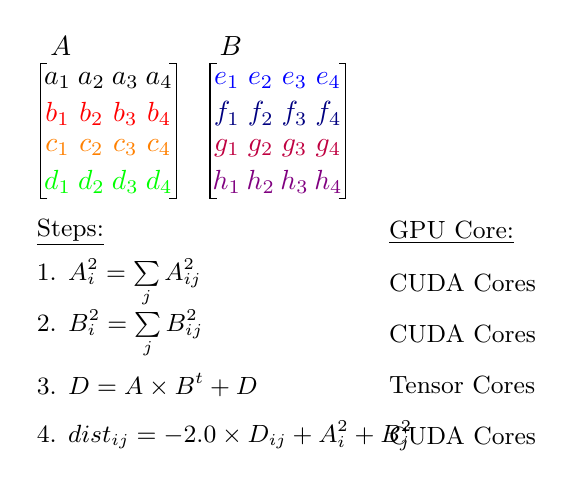
\begin{tikzpicture}[scale = 0.43]
\draw (5.2, 0) -- (5, 0) -- (5,4) -- (5.2, 4);
    \draw (8.8, 0) -- (9, 0) -- (9,4) -- (8.8, 4);
    \node[anchor=west] at (5, 4.5) {$A$};
        \node[] at (5.5, 3.5) {\color{black}$a_1$};
        \node[] at (6.5, 3.5) {\color{black}$a_2$};
        \node[] at (7.5, 3.5) {\color{black}$a_3$};
        \node[] at (8.5, 3.5) {\color{black}$a_4$};
        
        \node[] at (5.5, 2.5) {\color{red}$b_1$};
        \node[] at (6.5, 2.5) {\color{red}$b_2$};
        \node[] at (7.5, 2.5) {\color{red}$b_3$};
        \node[] at (8.5, 2.5) {\color{red}$b_4$};
        
        \node[] at (5.5, 1.5) {\color{orange}$c_1$};
        \node[] at (6.5, 1.5) {\color{orange}$c_2$};
        \node[] at (7.5, 1.5) {\color{orange}$c_3$};
        \node[] at (8.5, 1.5) {\color{orange}$c_4$};
        
        \node[] at (5.5, 0.5) {\color{green}$d_1$};
        \node[] at (6.5, 0.5) {\color{green}$d_2$};
        \node[] at (7.5, 0.5) {\color{green}$d_3$};
        \node[] at (8.5, 0.5) {\color{green}$d_4$};

    \draw (10.2, 0) -- (10, 0) -- (10,4) -- (10.2, 4);
    \draw (13.8, 0) -- (14, 0) -- (14,4) -- (13.8, 4);
    \node[anchor=west] at (10, 4.5) {$B$};
        \node[] at (10.5, 3.5) {\color{blue}$e_1$};
        \node[] at (11.5, 3.5) {\color{blue}$e_2$};
        \node[] at (12.5, 3.5) {\color{blue}$e_3$};
        \node[] at (13.5, 3.5) {\color{blue}$e_4$};
        
        \node[] at (10.5, 2.5) {\color{NavyBlue}$f_1$};
        \node[] at (11.5, 2.5) {\color{NavyBlue}$f_2$};
        \node[] at (12.5, 2.5) {\color{NavyBlue}$f_3$};
        \node[] at (13.5, 2.5) {\color{NavyBlue}$f_4$};
        
        \node[] at (10.5, 1.5) {\color{purple}$g_1$};
        \node[] at (11.5, 1.5) {\color{purple}$g_2$};
        \node[] at (12.5, 1.5) {\color{purple}$g_3$};
        \node[] at (13.5, 1.5) {\color{purple}$g_4$};
        
        \node[] at (10.5, 0.5) {\color{violet}$h_1$};
        \node[] at (11.5, 0.5) {\color{violet}$h_2$};
        \node[] at (12.5, 0.5) {\color{violet}$h_3$};
        \node[] at (13.5, 0.5) {\color{violet}$h_4$};
    
    

% \draw (15.2, 0) -- (15, 0) -- (15,4) -- (15.2, 4);
%\draw (18.8, 0) -- (19, 0) -- (19,4) -- (18.8, 4);
%\node[anchor=west] at (15, 4.5) {$P$: $A^2$};
%
%\node[] at (15.5, 3.5) {\color{black} $a^2_{1}$};
%\node[] at (16.5, 3.5) {\color{black} $a^2_2$};
%\node[] at (17.5, 3.5) {\color{black} $a^2_3$};
%\node[] at (18.5, 3.5) {\color{black} $a^2_4$};
%
%\node[] at (15.5, 2.5) {\color{red}$b^2_1$};
%\node[] at (16.5, 2.5) {\color{red}$b^2_2$};
%\node[] at (17.5, 2.5) {\color{red}$b^2_3$};
%\node[] at (18.5, 2.5) {\color{red}$b^2_4$};
%
%\node[] at (15.5, 1.5) {\color{orange}$c^2_1$};
%\node[] at (16.5, 1.5) {\color{orange}$c^2_2$};
%\node[] at (17.5, 1.5) {\color{orange}$c^2_3$};
%\node[] at (18.5, 1.5) {\color{orange}$c^2_4$};
%
%\node[] at (15.5, 0.5) {\color{green}$d^2_1$};
%\node[] at (16.5, 0.5) {\color{green}$d^2_2$};
%\node[] at (17.5, 0.5) {\color{green}$d^2_3$};
%\node[] at (18.5, 0.5) {\color{green}$d^2_4$};
%
%\draw (20.2, 0) -- (20, 0) -- (20,4) -- (20.2, 4);
%\draw (23.8, 0) -- (24, 0) -- (24,4) -- (23.8, 4);
%\node[anchor=west] at (20, 4.5) {$Q$: $(B^t)^2$};
%\node[] at (20.5, 3.5) {\color{blue}$e^2_1$};
%\node[] at (20.5, 2.5) {\color{blue}$e^2_2$};
%\node[] at (20.5, 1.5) {\color{blue}$e^2_3$};
%\node[] at (20.5, 0.5) {\color{blue}$e^2_4$};        
%
%\node[] at (21.5, 3.5) {\color{NavyBlue}$f^2_1$};
%\node[] at (21.5, 2.5) {\color{NavyBlue}$f^2_2$};
%\node[] at (21.5, 1.5) {\color{NavyBlue}$f^2_3$};
%\node[] at (21.5, 0.5) {\color{NavyBlue}$f^2_4$};

%\node[] at (22.5, 3.5) {\color{purple}$g^2_1$};
%\node[] at (22.5, 2.5) {\color{purple}$g^2_2$};
%\node[] at (22.5, 1.5) {\color{purple}$g^2_3$};
%\node[] at (22.5, 0.5) {\color{purple}$g^2_4$};
%
%\node[] at (23.5, 3.5) {\color{violet}$h^2_1$};
%\node[] at (23.5, 2.5) {\color{violet}$h^2_2$};
%\node[] at (23.5, 1.5) {\color{violet}$h^2_3$};
%\node[] at (23.5, 0.5) {\color{violet}$h^2_4$};




    \node[anchor=west] at (4.6, -1) {\small{\underline{Steps:}}};
    \node[anchor=west] at (4.6, -2.5) {\small{1. $A_i^2 = \sum\limits_j{A_{ij}^2}$}};
    \node[anchor=west] at (4.6, -4.0) {\small{2. $B_i^2 = \sum\limits_j{B_{ij}^2}$}};
    \node[anchor=west] at (4.6, -5.5) {\small{3. $D = A \times B^{t} + D$}};
    \node[anchor=west] at (4.6, -7.0) {\small{4. $dist_{ij} = -2.0 \times D_{ij} + A_i^2 + B_j^2$}};

    \node[anchor=west] at (15, -1) {\small{\underline{GPU Core:}}};
    \node[anchor=west] at (15, -2.5) {\small{CUDA Cores}};
    \node[anchor=west] at (15, -4.0) {\small{CUDA Cores}};
    \node[anchor=west] at (15, -5.5) {\small{Tensor Cores}};
    \node[anchor=west] at (15, -7.0) {\small{CUDA Cores}};
    
\end{tikzpicture}

    \vspace*{-0.2cm}
    \caption{Outline of Euclidean distance calculations on tensor cores. For illustrative purposes we show 4$\times$4 matrices; however, the actual $A$ matrix is 16$\times$16 and the actual $B$ matrix is 16$\times$8. For clarity, the coordinates of a given point are shown using the same color.}
    \label{fig:euclidean_distance_TC_overview}
\end{figure}






% We provide a brief overview of how we are computing Euclidean distances on TCs. 
% \brian{Should we call out that what we are doing is a bit different when we refer to prior work? Like we are not planning on short circuiting so that we can have less computation cycles.}
% \brian{We should just remove the reference to the other work and say how we are doing it.}
As an illustrative example, Figure~\ref{fig:euclidean_distance_TC_overview} shows the calculation of Euclidean distances in $d=4$ dimensions, where the distances between points $a, b, c, d$ and $e, f, g, h$ are computed. Thus, the computation results in a total of 16 Euclidean distances between the two sets of four points. 

Referring to Figure~\ref{fig:euclidean_distance_TC_overview}, we store in row-major order the coordinates of points $a, b, c, d$ in matrix $A$ and the coordinates of points $e, f, g, h$ in matrix $B$, and then we perform the following steps. {\bf Step~1:} On CUDA cores, we pre-compute the sum of the squared values in each row of matrix $A$ and store it in global memory. {\bf Step~2:} We do the same for matrix $B$. {\bf Step~3:} The matrix $D$ is initialized with zeros, and then we use TCs to compute $D = A \times B^{t} + D$ over many iterations.  We only show $4$ dimensional data for illustrative purposes, but in practice we need to accumulate into $D$ across multiple iterations because TCs can only compute inner products in 16 dimensions. {\bf Step~4:} Once this is complete, the results $D_{ij}$ are multiplied by $-2.0$, and their corresponding sum of squared terms (steps 1--2) are added. This has computed $-2ab+a^2+b^2$ (Equation~\ref{eqn:euclidean_distance_TCs}). 

From Figure~\ref{fig:euclidean_distance_TC_overview}, steps~1, 2, and 4 require significantly less work than step~3, and so we elect to compute these steps on CUDA cores. While these steps can be computed on TCs, it would require MMA operations that are much more expensive than simple operations on CUDA cores.

\subsection{Overview of the Data Path from Global Memory to Registers}\label{sec:mptc_overview_data_path}
% \subsection{Overview of Optimizations}
\mike{I changed the subsection title. We can work on rewording this.}
While the basic algorithm to compute Euclidean distances using TCs is straightforward conceptually, computing step~3 in Figure~\ref{fig:euclidean_distance_TC_overview} with high throughput is challenging. The Nvidia A100 GPU that we use in the evaluation boasts a peak throughput of 312 TFLOPS in FP16-32. Previous GPU work that computed distance similarity searches focused on algorithmic optimizations using indexed search methods to reduce the search space, as well as short circuiting techniques to reduce computation (Section~\ref{sec:background_tedjoin}--\ref{sec:related_work_gpu_similarity_searches}). However, to utilize their claimed throughput, TCs need a well organized and balanced workload that these index-supported algorithms can not provide (i.e., they perform a higher ratio of memory operations compared to computation operations and have more non-deterministic execution pathways that cause warp divergence). To achieve high throughput, we propose a significant number of optimizations that aim to deliver the data to the TCs as fast as possible to mitigate underutilization.

\mike{Need to walk the reader through Figures~\ref{fig:single_mma}-\ref{fig:entire_mma}}
Figures~\ref{fig:single_mma}--\ref{fig:entire_mma} show how a single 16$\times$8$\times$16 MMA operation can be used to compute an even larger and deeper ``warp tile'', and how multiple warp tiles can be combined and run over many iterations into a ``block tile'' that can compute the final distance matrix $D$.

\begin{figure}[!t]
    \centering
    

% Basic TC MMA
\begin{tikzpicture}
	\newcommand\fm{4.5}
	\newcommand\fn{3}
	\newcommand\fk{4.5}

		% Draw B
	\pgfmathsetmacro\bdXShift{1.5}
	\draw[style=fragment,draw=BFragmentColor, ultra thick] (0, 0) rectangle +(\fn, -\fk);
	\matrix (m) [xshift=\bdXShift cm, yshift=-2.25cm, 
	matrix of math nodes,
	row sep=0.5em, column sep=0em,
	nodes={anchor=center}] {
		C_{1,1} & \cdots & C_{8,1} \\
		C_{1,2} & \cdots & C_{8,2} \\
		\vdots & \ddots & \vdots \\
		C_{1,15} & \cdots & C_{8,15} \\
		C_{1,16} & \cdots & C_{8,16} \\
	};

		% Draw D
	\pgfmathsetmacro\dXShift{0}
	\pgfmathsetmacro\dYShift{-\whiteSpace - \fk}
	\draw[style=fragment,draw=DFragmentColor, xshift=\dXShift cm, yshift=\dYShift cm, ultra thick] (0, 0) rectangle +(\fn, -\fm);
	\pgfmathsetmacro\adYShift{-7.25}
	\matrix (m) [xshift=\bdXShift cm, yshift=\adYShift cm, 
	matrix of math nodes,
	row sep=0.5em, column sep=0em,
		%left delimiter={[}, right delimiter={]},
	nodes={anchor=center}] {
		D_{1,1} & \cdots & D_{1,8} \\
		D_{2,1} & \cdots & D_{2,8} \\
		\vdots & \ddots & \vdots \\
		D_{15,1} & \cdots & D_{15,8} \\
		D_{16,1} & \cdots & D_{16,8} \\
	};

		% Draw A
	\pgfmathsetmacro\aXShift{-\whiteSpace - \fk}
	\pgfmathsetmacro\aYShift{-\whiteSpace - \fm}
	\draw[style=fragment,draw=AFragmentColor, xshift=\aXShift cm, yshift=\aYShift cm, ultra thick] (0, 0) rectangle +(\fk, -\fm);
	\matrix (m) [xshift=-2.75 cm, yshift=\adYShift cm, 
	matrix of math nodes,
	row sep=0.5em, column sep=0.5em,
	nodes={anchor=center}] {
		Q_{1,1} & Q_{1,2} & \cdots & Q_{1,16} \\
		Q_{2,1} & Q_{2,2} & \cdots & Q_{2,16} \\
		\vdots & \vdots & \ddots & \vdots \\
		Q_{15,1} & Q_{15,2} & \cdots & Q_{15,16} \\
		Q_{16,1} & Q_{16,2} & \cdots & Q_{16,16} \\
	};

\end{tikzpicture}

    \caption{A single 16$\times$8$\times$16 Tensor core computation, as executed by inline PTX instructions. Shows a single fragment for A (candidate points in red), B (query points in blue), and D (distances in green). Performs $D=A\times B+D$.}
    \label{fig:single_mma}
    \mike{In all of the tikz figures is there extra space at the bottom of the figures? The captions have a large space between them and the images.}
\end{figure}

\begin{figure}[!t]
    \centering
    \documentclass[tikz,border=2mm]{standalone}

% Binary value zero padding taken from SO
\ExplSyntaxOn
\int_new:N \g_fleet_number_of_zeros
\NewDocumentCommand\SetZeros{m}
{
	\int_gset:Nn \g_fleet_number_of_zeros {#1}
}
\NewDocumentCommand\PrependZeros{om}
{
	\IfValueTF{#1}
	{ \__fleet_count:ne {#1} {#2} }
	{ \__fleet_count:ne {\g_fleet_number_of_zeros} {#2} }
}
\cs_new:Npn \__fleet_count:nn #1#2
{
	\exp_args:Nf \__fleet_prepend:nn
	{ \int_max:nn { #1 - \str_count:n {#2} } { 0 } }
	{#2}
}
\cs_generate_variant:Nn \__fleet_count:nn { ne }
\cs_new:Npn \__fleet_prepend:nn #1#2
{ \prg_replicate:nn {#1}{0} #2 }
\ExplSyntaxOff

% XOR routine taken from SO...
\ExplSyntaxOn
\NewExpandableDocumentCommand{\bitwiseXor}{mm}
{
	\recuenco_bitwise_xor:nn { #1 } { #2 }
}

\cs_new:Nn \recuenco_bitwise_xor:nn
{
	\int_from_bin:e
	{
		\__recuenco_bitwise_xor:ee { \int_to_bin:n { #1 } } { \int_to_bin:n { #2 } }
	}
}
\cs_generate_variant:Nn \int_from_bin:n { e }

\cs_new:Nn \__recuenco_bitwise_xor:nn
{
	\__recuenco_bitwise_xor_binary:ee
	{
		\prg_replicate:nn
		{
			\int_max:nn { \tl_count:n { #1 } } { \tl_count:n { #2 } } - \tl_count:n { #1 }
		}
		{ 0 }
		#1
	}
	{
		\prg_replicate:nn
		{
			\int_max:nn { \tl_count:n { #1 } } { \tl_count:n { #2 } } - \tl_count:n { #2 }
		}
		{ 0 }
		#2
	}
}
\cs_generate_variant:Nn \__recuenco_bitwise_xor:nn { ee }

\cs_new:Nn \__recuenco_bitwise_xor_binary:nn
{
	\__recuenco_bitwise_xor_binary:w #1;#2;
}
\cs_generate_variant:Nn \__recuenco_bitwise_xor_binary:nn { ee }

\cs_new:Npn \__recuenco_bitwise_xor_binary:w #1#2;#3#4;
{
	\int_abs:n { #1-#3 }
	\tl_if_empty:nF { #2 } { \__recuenco_bitwise_xor_binary:w #2;#4; }
}

\ExplSyntaxOff


\definecolor{colColor0}{RGB}{255, 102, 102} % Soft Red  
\definecolor{colColor1}{RGB}{255, 140, 115} % Coral  
\definecolor{colColor2}{RGB}{255, 178, 140} % Soft Orange  
\definecolor{colColor3}{RGB}{230, 153, 190} % Warm Pink  
\definecolor{colColor4}{RGB}{200, 130, 220} % Light Orchid  
\definecolor{colColor5}{RGB}{170, 110, 230} % Soft Violet  
\definecolor{colColor6}{RGB}{140, 90, 240}  % Muted Purple  
\definecolor{colColor7}{RGB}{120, 70, 250}  % Gentle Blue-Purple  
\definecolor{lastColColor}{RGB}{255, 255, 255}  % White
\definecolor{AFragmentColor}{RGB}{255, 0, 0}  % Red
\definecolor{BFragmentColor}{RGB}{0, 0, 255}  % Blue
\definecolor{DFragmentColor}{RGB}{0, 203, 74}  % Green
\definecolor{ASharedMemColor}{RGB}{200, 0, 0}  % Red
\definecolor{BSharedMemColor}{RGB}{0, 0, 200}  % Blue
\definecolor{WarpTileColor}{RGB}{0, 150, 74}  % Green
\definecolor{BlockTileColor}{RGB}{0, 0, 0}  % Black

\definecolor{blockTileColor}{RGB}{0, 255, 0}  % Light Green

\newcommand{\getcolor}[1]{colColor#1}


\def\blockHeight{1}
\def\blockWidth{2}
\pgfmathsetmacro{\halfBlockHeight}{\blockHeight / 2}
\pgfmathsetmacro{\halfBlockWidth}{\blockWidth / 2}

\def\dimColors{colColor0, colColor1, colColor2, colColor3, colColor4, colColor5, colColor6, colColor7, lastColColor}

% Fragment drawings common parameters

% Base rectangle background
\newcommand\whiteSpace{0.5}

	% Compute width of a single register based on the fraction of a single chunk it takes up.
\pgfmathsetmacro\registerWidth{0.75}
\pgfmathsetmacro\registerHeight{0.375}
\pgfmathsetmacro\halfRegisterWidth{\registerWidth / 2}
\pgfmathsetmacro\halfRegisterHeight{\registerHeight / 2}

\newcommand\phasesPercent{0.8}
\pgfmathsetmacro\phaseWidth{\registerWidth * 4}
\pgfmathsetmacro\phaseHeight{\registerHeight * 8}

\pgfmathsetmacro\fragmentWidth{2 * \phaseWidth + (3 * \whiteSpace)}
\pgfmathsetmacro\fragmentHeight{2 * \phaseHeight + (3 * \whiteSpace)}

\tikzstyle fragment=[ultra thick, rounded corners= 5pt]

\newcommand\drawFragment[1]{
	\draw[style=fragment, draw=AFragmentColor] (0, 0) rectangle +(\fragmentWidth, -\fragmentHeight);

	\begin{scope}[xshift=\whiteSpace cm, yshift=-\whiteSpace cm]

	% Draw the four phases
		\foreach \row in {0,  1} {
			\foreach \col in {0,  1} {
				\pgfmathsetmacro\xoffset{\col * (\phaseWidth + \whiteSpace)}
				\pgfmathsetmacro\yoffset{-\row * (\phaseHeight + \whiteSpace)}
				\begin{scope}[xshift=\xoffset cm, yshift=\yoffset cm]
					\pgfmathsetmacro\phaseNum{int(\col * 2 + \row + 1)}
					\node[anchor=south] at (\registerWidth * 2, 0) {Phase \phaseNum};
					% Invoke the Phase drawing section now that we are in our local scope
					#1{\phaseNum}
				\end{scope}
			}
		}
	\end{scope}
}

\newcommand\getPhaseColor[1]{%
	\ifcase #1 \or colColor0%
		\or white%
		\or colColor1%
		\or white%
	\fi
}


\begin{document}
% Warp Tile
\begin{tikzpicture}[show background rectangle, 
    background rectangle/.style={style=fragment, fill=WarpTileColor}]
	\newcommand\drawStackableFragment[6]{%
		\def\width{#1}
		\def\height{#2}
		\def\upperLeftContent{#3}
		\def\bottomRightContent{#4}
		\def\singlefragcolor{#5}
            \def\label{#6}

            \def\labelShift{0.8}

		\filldraw[style=fragment, fill=\singlefragcolor, draw=black] (0, 0) node[anchor=south east,  font=\tiny, xshift=0.5 mm, yshift=-\labelShift mm, text=white] {\bottomRightContent} rectangle (-\width, \height) node[anchor=north west,  yshift=\labelShift mm, font=\tiny, text=white] {\upperLeftContent} node[midway,  align=center, font=\scriptsize, text=white] {\label};
	}


	\newcommand\fullFragWidth{1.5}
	\pgfmathsetmacro\fullFragHeight{\fullFragWidth}
	\pgfmathsetmacro\halfFragWidth{\fullFragWidth / 2}
	\newcommand\halfFragPoints{8}
	\newcommand\fullFragPoints{16}
	% All fragments have 16 dimensions
	\newcommand\fragmentDims{16}

	% Can be used to draw stacks of fragments for A or B matrices
	\newcommand\drawFragmentStack[6]{%
		\def\fragColor{#1}
		\def\fragWidth{#2}
		\def\fragWidthInPoints{#3}
		\def\fragIndex{#4}
		\def\fragName{#5}
            % Center label
		\def\fragLabel{#6}

		% Draw each fragment as a stack 
		\newcommand\stacks{2}
		\newcommand\stackOffset{0.325}
		\pgfmathsetmacro\maxStackIndex{int(\stacks - 1)}

		\foreach \i in {0, ..., \maxStackIndex} {
			% Stack up and to the left
			\begin{scope}[xshift=-\i * \stackOffset * 0.125 cm, yshift=\i * \stackOffset cm]
				\pgfmathtruncatemacro\minPoint{\fragWidthInPoints * \fragIndex + 1}
				\pgfmathtruncatemacro\maxPoint{\minPoint + \fragWidthInPoints - 1}

																% Kind of a hack, but we stack upwards so later fragments cover earlier, have
																% to count backwards for dimensions for this to work out cleanly
				\pgfmathtruncatemacro\maxDim{\fragmentDims * \stacks - (\i * \fragmentDims)}
				\pgfmathtruncatemacro\minDim{\maxDim - \fragmentDims + 1}

				\drawStackableFragment{\fragWidth}{\fullFragHeight}{$\fragName_{\minPoint,\minDim}$}{$\fragName_{\maxPoint,\maxDim}$}{\fragColor}{\fragLabel}
			\end{scope}
		}
	}


	\newcommand\fragXShift{1.0}
	\newcommand\fragYShift{2.0}
	\newcommand\numAFragments{2}
	\pgfmathtruncatemacro\aFragmentsMaxIndex{\numAFragments - 1}
	\newcommand\numBFragments{4}
	\pgfmathtruncatemacro\bFragmentsMaxIndex{\numBFragments - 1}

	% Draw all D Fragments
	\begin{scope}[xshift=1 cm, yshift=0 cm]
		\foreach \row in {0, ..., \aFragmentsMaxIndex} {
			\foreach \col in {0, ..., \bFragmentsMaxIndex} {
				\begin{scope}[xshift=\fragXShift * \col cm, yshift= -\fragYShift * \row cm]
					\pgfmathtruncatemacro\firstQueryPoint{\row * \fullFragPoints + 1}
					\pgfmathtruncatemacro\lastQueryPoint{\firstQueryPoint + \fullFragPoints - 1}
					\pgfmathtruncatemacro\firstCandPoint{\col * \halfFragPoints + 1}
					\pgfmathtruncatemacro\lastCandPoint{\firstCandPoint + \halfFragPoints - 1}

					\drawStackableFragment{\halfFragWidth}{\fullFragHeight}{$a_{\firstQueryPoint,\firstCandPoint}$}{$a_{\lastQueryPoint,\lastCandPoint}$}{DFragmentColor}{\arf}
				\end{scope}
			}
		}
	\end{scope}

	% Draw all 2 A Fragments
	\begin{scope}[xshift=0 cm, yshift=0 cm]
		\foreach \fragment in {0, ..., \aFragmentsMaxIndex} {
			\begin{scope}[yshift=-\fragYShift * \fragment cm]
				\drawFragmentStack{AFragmentColor}{\fullFragWidth}{16}{\fragment}{p}{\prf}
			\end{scope}
		}
	\end{scope}

	% Draw all 4 B Fragments
	\begin{scope}[xshift=1 cm, yshift=1.75 cm]
		\foreach \fragment in {0, ..., \bFragmentsMaxIndex} {
			\begin{scope}[xshift=\fragXShift * \fragment cm]
				\drawFragmentStack{BFragmentColor}{\halfFragWidth}{8}{\fragment}{p}{\qrf}
			\end{scope}
		}

	\end{scope}

  % Draw the entire warp tile for future reference
	\drawLabeledBoundingBox{color=WarpTileColor}{Single Warp Tile}{black}

\end{tikzpicture}
\end{document}

    \caption{A single warp iteratively transfers a single 16-D ``k-slice'' fragments from shared memory, multiplies all the fragments of A and B by each other, accumulates the results, and repeats this for four different 16-D ``k-slices''. This sequence computes a $48\times48\times64$ ``warp tile''. Once the four iterations are complete and the next set of operands has finished being transferred into shared memory through the multi-stage pipeline, this operation is repeated. This sequence repeats until all k-dimensions have been accumulated.}
    \label{fig:warp_mma}
\end{figure}

\begin{figure}[!t]
    \centering
    

% Block Tile last one!!!
\begin{tikzpicture}

	\newcommand\drawBlockLevelFragment[6]{%
		\def\width{#1}
		\def\height{#2}
		\def\upperLeftContent{#3}
		\def\bottomRightContent{#4}
		\def\color{#5}
		\def\label{#6}

		\filldraw[style=fragment, fill= white, draw=\color] (0, 0) node[anchor=south east, font=\small] {\bottomRightContent} rectangle (-\width, \height) node[anchor=north west, font=\small] {\upperLeftContent} node[midway, align=center, font=\small] {\label};
	}

% Draw the entire block tile
	\draw[color=BlockTileColor, style=fragment, xshift=-9 cm, yshift=10 cm] (0,0) rectangle (15, -16) node[anchor=south east] {Single Block Tile};

	% Draw the 4 warp tiles in center
	\newcommand\warpTileSize{4}
	\newcommand\warpPadding{1}
	\pgfmathtruncatemacro\paddedWarpTileSize{\warpTileSize + \warpPadding}


	% Draw all Warp Tiles
	\begin{scope}[xshift=0 cm, yshift=0 cm]
		\foreach \row in {0, ..., 1} {
			\foreach \col in {0, ..., 1} {
				\begin{scope}[xshift=\paddedWarpTileSize * \col cm, yshift= -\paddedWarpTileSize * \row cm]
					\pgfmathtruncatemacro\warpIndex{\row * 2 + \col + 1}
					\pgfmathtruncatemacro\warpSize{48}

					\pgfmathtruncatemacro\minQueryPoint{\row * \warpSize + 1}
					\pgfmathtruncatemacro\maxQueryPoint{\minQueryPoint + \warpSize - 1}
					\pgfmathtruncatemacro\minCandPoint{\col * \warpSize + 1}
					\pgfmathtruncatemacro\maxCandPoint{\minCandPoint + \warpSize - 1}
					\def\minDim{1}
					\def\maxDim{64}

					\drawBlockLevelFragment{\warpTileSize}{\warpTileSize}{$D_{\minQueryPoint,\minCandPoint}$}{$D_{\maxQueryPoint,\maxCandPoint}$}{WarpTileColor}{Warp Tile\\ \warpIndex}
				\end{scope}
			}
		}
	\end{scope}

	\def\sliceYShift{0.55}
	\def\sliceXShift{0.25}
	\pgfmathtruncatemacro\numSlices{3 - 1}
	% Draw the 64D shared memory chunks that have been paged in
	% A Data
	\begin{scope}[xshift=-5 cm, yshift=-5 cm]
		\foreach \i in {0, ..., \numSlices} {
			\begin{scope}[xshift=-\sliceXShift * \i cm, yshift=\sliceYShift * \i cm]
				\pgfmathtruncatemacro\maxDim{64 * 3 - 64 * \i}
				\drawBlockLevelFragment{\warpTileSize * 0.75}{2 * \warpTileSize + \warpPadding}{$Q_{1,1}$}{$Q_{96,\maxDim}$}{ASharedMemColor}{Query Points\\ 64D k-slice\\ (SMEM)}
			\end{scope}
		}
	\end{scope}

	% B Data
	\begin{scope}[xshift=5 cm, yshift=5 cm]
		\pgfmathsetmacro\blockWidth{2 * \warpTileSize + \warpPadding}
		\foreach \i in {0, ..., \numSlices} {
			\begin{scope}[xshift=-\sliceXShift * \i cm, yshift=\sliceYShift * \i cm]
				\pgfmathtruncatemacro\maxDim{64 * 3 - 64 * \i}
		\drawBlockLevelFragment{\blockWidth}{\warpTileSize * 0.75}{$C_{1,1}$}{$C_{96,\maxDim}$}{BSharedMemColor}{Candidate Points\\ 64D k-slice (SMEM)}
			\end{scope}
		}
	\end{scope}

\end{tikzpicture}

    \caption{A single block iteration transfers in two 64-D k-slices of point data (A and B) at a time from global memory to shared memory. Four ``warp tiles'' (Figure~\ref{fig:warp_mma}) each page a portion of that data into their own registers, and accumulate the distances. This sequence is repeated for $\frac{|D|}{64}$ iterations and computes a $96\times96$ ``block tile'' of the final distances.}
    \label{fig:block_tile_mma}
\end{figure}

\begin{figure}[!t]
    \centering
    \documentclass[tikz,border=2mm]{standalone}

% Binary value zero padding taken from SO
\ExplSyntaxOn
\int_new:N \g_fleet_number_of_zeros
\NewDocumentCommand\SetZeros{m}
{
	\int_gset:Nn \g_fleet_number_of_zeros {#1}
}
\NewDocumentCommand\PrependZeros{om}
{
	\IfValueTF{#1}
	{ \__fleet_count:ne {#1} {#2} }
	{ \__fleet_count:ne {\g_fleet_number_of_zeros} {#2} }
}
\cs_new:Npn \__fleet_count:nn #1#2
{
	\exp_args:Nf \__fleet_prepend:nn
	{ \int_max:nn { #1 - \str_count:n {#2} } { 0 } }
	{#2}
}
\cs_generate_variant:Nn \__fleet_count:nn { ne }
\cs_new:Npn \__fleet_prepend:nn #1#2
{ \prg_replicate:nn {#1}{0} #2 }
\ExplSyntaxOff

% XOR routine taken from SO...
\ExplSyntaxOn
\NewExpandableDocumentCommand{\bitwiseXor}{mm}
{
	\recuenco_bitwise_xor:nn { #1 } { #2 }
}

\cs_new:Nn \recuenco_bitwise_xor:nn
{
	\int_from_bin:e
	{
		\__recuenco_bitwise_xor:ee { \int_to_bin:n { #1 } } { \int_to_bin:n { #2 } }
	}
}
\cs_generate_variant:Nn \int_from_bin:n { e }

\cs_new:Nn \__recuenco_bitwise_xor:nn
{
	\__recuenco_bitwise_xor_binary:ee
	{
		\prg_replicate:nn
		{
			\int_max:nn { \tl_count:n { #1 } } { \tl_count:n { #2 } } - \tl_count:n { #1 }
		}
		{ 0 }
		#1
	}
	{
		\prg_replicate:nn
		{
			\int_max:nn { \tl_count:n { #1 } } { \tl_count:n { #2 } } - \tl_count:n { #2 }
		}
		{ 0 }
		#2
	}
}
\cs_generate_variant:Nn \__recuenco_bitwise_xor:nn { ee }

\cs_new:Nn \__recuenco_bitwise_xor_binary:nn
{
	\__recuenco_bitwise_xor_binary:w #1;#2;
}
\cs_generate_variant:Nn \__recuenco_bitwise_xor_binary:nn { ee }

\cs_new:Npn \__recuenco_bitwise_xor_binary:w #1#2;#3#4;
{
	\int_abs:n { #1-#3 }
	\tl_if_empty:nF { #2 } { \__recuenco_bitwise_xor_binary:w #2;#4; }
}

\ExplSyntaxOff


\definecolor{colColor0}{RGB}{255, 102, 102} % Soft Red  
\definecolor{colColor1}{RGB}{255, 140, 115} % Coral  
\definecolor{colColor2}{RGB}{255, 178, 140} % Soft Orange  
\definecolor{colColor3}{RGB}{230, 153, 190} % Warm Pink  
\definecolor{colColor4}{RGB}{200, 130, 220} % Light Orchid  
\definecolor{colColor5}{RGB}{170, 110, 230} % Soft Violet  
\definecolor{colColor6}{RGB}{140, 90, 240}  % Muted Purple  
\definecolor{colColor7}{RGB}{120, 70, 250}  % Gentle Blue-Purple  
\definecolor{lastColColor}{RGB}{255, 255, 255}  % White
\definecolor{AFragmentColor}{RGB}{255, 0, 0}  % Red
\definecolor{BFragmentColor}{RGB}{0, 0, 255}  % Blue
\definecolor{DFragmentColor}{RGB}{0, 203, 74}  % Green
\definecolor{ASharedMemColor}{RGB}{200, 0, 0}  % Red
\definecolor{BSharedMemColor}{RGB}{0, 0, 200}  % Blue
\definecolor{WarpTileColor}{RGB}{0, 150, 74}  % Green
\definecolor{BlockTileColor}{RGB}{0, 0, 0}  % Black

\definecolor{blockTileColor}{RGB}{0, 255, 0}  % Light Green

\newcommand{\getcolor}[1]{colColor#1}


\def\blockHeight{1}
\def\blockWidth{2}
\pgfmathsetmacro{\halfBlockHeight}{\blockHeight / 2}
\pgfmathsetmacro{\halfBlockWidth}{\blockWidth / 2}

\def\dimColors{colColor0, colColor1, colColor2, colColor3, colColor4, colColor5, colColor6, colColor7, lastColColor}

% Fragment drawings common parameters

% Base rectangle background
\newcommand\whiteSpace{0.5}

	% Compute width of a single register based on the fraction of a single chunk it takes up.
\pgfmathsetmacro\registerWidth{0.75}
\pgfmathsetmacro\registerHeight{0.375}
\pgfmathsetmacro\halfRegisterWidth{\registerWidth / 2}
\pgfmathsetmacro\halfRegisterHeight{\registerHeight / 2}

\newcommand\phasesPercent{0.8}
\pgfmathsetmacro\phaseWidth{\registerWidth * 4}
\pgfmathsetmacro\phaseHeight{\registerHeight * 8}

\pgfmathsetmacro\fragmentWidth{2 * \phaseWidth + (3 * \whiteSpace)}
\pgfmathsetmacro\fragmentHeight{2 * \phaseHeight + (3 * \whiteSpace)}

\tikzstyle fragment=[ultra thick, rounded corners= 5pt]

\newcommand\drawFragment[1]{
	\draw[style=fragment, draw=AFragmentColor] (0, 0) rectangle +(\fragmentWidth, -\fragmentHeight);

	\begin{scope}[xshift=\whiteSpace cm, yshift=-\whiteSpace cm]

	% Draw the four phases
		\foreach \row in {0,  1} {
			\foreach \col in {0,  1} {
				\pgfmathsetmacro\xoffset{\col * (\phaseWidth + \whiteSpace)}
				\pgfmathsetmacro\yoffset{-\row * (\phaseHeight + \whiteSpace)}
				\begin{scope}[xshift=\xoffset cm, yshift=\yoffset cm]
					\pgfmathsetmacro\phaseNum{int(\col * 2 + \row + 1)}
					\node[anchor=south] at (\registerWidth * 2, 0) {Phase \phaseNum};
					% Invoke the Phase drawing section now that we are in our local scope
					#1{\phaseNum}
				\end{scope}
			}
		}
	\end{scope}
}

\newcommand\getPhaseColor[1]{%
	\ifcase #1 \or colColor0%
		\or white%
		\or colColor1%
		\or white%
	\fi
}


\begin{document}


% Block Tile Rasterization
\begin{tikzpicture}
	\newcommand\tileSpacing{0.25}
	\newcommand\tileDim{0.6}
    
	% Draw global memory layouts
	\newcommand\kHeight{1}
	\pgfmathsetmacro\mHeight{4 * \tileDim + 3 * \tileSpacing}
	\tikzstyle nodeStyle=[align=center, font=\footnotesize]
        \pgfmathsetmacro\queryXOffset{-\kHeight - \tileSpacing}
	\filldraw[xshift=\queryXOffset cm, yshift=0 cm, style=fragment, fill=GlobalPointsColor] (0, 0) rectangle +(\kHeight, -\mHeight) node[midway, style=nodeStyle] {Points\\ (DRAM)};
	\filldraw[xshift=0 cm, yshift=0.25 cm, style=fragment, fill=GlobalQueriesColor] (0, \kHeight) rectangle +(\mHeight, -\kHeight) node[midway, style=nodeStyle] {Query Points\\ (DRAM)};


	\pgfmathsetmacro\paddedTileDim{\tileDim + \tileSpacing}

		% Remember the last node that we need to draw an arrow from
	\def\innerTiles{2}
	\def\outerChunks{2}

		% Outer square rasterized chunks
	\pgfmathsetmacro\outerRange{int(\outerChunks - 1)}

	\foreach \outerRow in {0, ..., \outerRange} {
		\foreach \outerCol in {0, ..., \outerRange} {
			\pgfmathsetmacro\outerIndex{int(\outerRow * \outerChunks + \outerCol)}
			\begin{scope}[xshift=\outerCol * \innerTiles * \paddedTileDim cm,
				yshift=-\outerRow * \innerTiles * \paddedTileDim cm]

				% inner square rasterized chunks
				\pgfmathsetmacro\innerRange{int(\innerTiles - 1)}
				\foreach \row in {0, ..., \innerRange} {
					\foreach \col in {0, ..., \innerRange} {
						\pgfmathsetmacro\innerIndex{int(\row * \innerTiles + \col + 1)}
						\pgfmathsetmacro\tileIndex{int(\outerIndex * (\innerTiles * \innerTiles) + \innerIndex)}

						\coordinate (TileUL) at (\col * \paddedTileDim, -\row * \paddedTileDim);
						\filldraw[style=fragment, fill=BlockTileColor] (TileUL) rectangle ++(\tileDim, -\tileDim) node[midway, font=\tiny, align=center, color=black] {Block\\ Tile \tileIndex};

																		% Compute left and right nodes for arrows
						\coordinate (currentRightNode) at ($(TileUL) + (\tileDim, -\tileDim / 2)$);
						\coordinate (currentLeftNode) at ($(TileUL) + (0, -\tileDim / 2)$);
						\coordinate (currentBottomNode) at ($(TileUL) + (\tileDim / 2, -\tileDim)$);
						\coordinate (currentTopNode) at ($(TileUL) + (\tileDim / 2, 0)$);
						\tikzstyle arrow=[rounded corners=1pt, arrows=-{Latex[width=1.0mm, length=1.0mm]}]
																% Draw connecting arrows
						\newcommand\arrowOffset{\tileSpacing / 2}

						\newcommand\drawOuterShortArrow{
							\ifnum \innerIndex=1
								\draw[style=arrow] (lastRightNode) -- ++(\arrowOffset, 0) -- ++(0, \innerTiles * \paddedTileDim - \paddedTileDim) -- ++(\arrowOffset, 0);
							\fi
						}
						\newcommand\drawOuterLongArrow{
							\ifnum \innerIndex=1
								\draw[style=arrow] (lastBottomNode) -- ++(0 , -\tileSpacing / 2) -- ++(-4 * \paddedTileDim + \paddedTileDim, 0) -- ++(0, -\arrowOffset);
							\fi
						}
																		% Draw outer-raster-square connecting arrows
						\ifnum \outerIndex=1
							\drawOuterShortArrow{}
						\fi
						\ifnum \outerIndex=2
							\drawOuterLongArrow{}
						\fi
						\ifnum \outerIndex=3
							\drawOuterShortArrow{}
						\fi
																		% Draw normal inner connecting arrows
						\ifnum \col>0
							\draw[style=arrow] (lastRightNode) -- +(\tileSpacing, 0);
						\fi
																		% Draw last to first connecting arrows
						\ifnum \col=0
							\ifnum \row>0
								\draw[style=arrow] (lastBottomNode) -- ++(0, -\tileSpacing / 2) -- ++(-\innerTiles * \paddedTileDim + \paddedTileDim, 0) -- ++(0 , -\tileSpacing / 2);
							\fi
						\fi

																		% Save the last right node for the next iteration to connect
																		% arrows to it
						\coordinate (lastLeftNode) at (currentLeftNode);
						\coordinate (lastRightNode) at (currentRightNode);
						\coordinate (lastTopNode) at (currentTopNode);
						\coordinate (lastBottomNode) at (currentBottomNode);

					}
				}
			\end{scope}
		}
	}

\end{tikzpicture}
\end{document}

    \caption{The entire dataset is first transferred to global memory, and then four times as many blocks as there are SMs on the GPU are launched to saturate GPU resources and hide latency. Each block computes a single 96$\times$96 tile of distances at a time. The coordinates of the tile are specified by a work dispatcher that orders computation into small rasterized squares to create L2 cache hits and increase the memory transfer rate.}
    \label{fig:entire_mma}
\end{figure}


\subsection{Mixed Precision Tensor Cores}
Previous work has used single-precision CUDA cores, as well as double-precision tensor cores. On Ampere GPUs, Tensor Cores can use half precision (FP16) operands, and accumulate in single precision (FP32). This configuration saves shared memory and register usage to store the operands and offers a 16x speedup over CUDA cores and Tensor cores. The accuracy trade-off from higher precision operands is investigated later.
\brian{Would it make more sense to move this earlier somewhere? It doesn't quite fit here, and in the intro we could probably say how we are going to use mixed precision computation.}
\mike{I think we can remove this because we already discussed it in the introduction in the paragraph that starts with "Peak throughput, defined here as the maximum number of Tera Floating Point Operations Per Second..." }


% \subsection{Hierarchical Memory Reuse and Optimization}
\subsection{Optimizations: Mitigating the Memory Bottleneck}
\mike{I changed the subsection title}
\mike{"while respecting the limited global memory, shared memory, and register capacities." Should this be capacities here? I changed it to this, but I wasn't certain if that's what you meant.}
As described in Section~\ref{sec:mptc_overview_data_path}, the Nvidia A100 has a peak performance using FP16-32 of 312 TFLOPS.
Consider that for every two FLOPS of the 312 TFLOPS, two 2 byte (FP16) elements must be stored in registers on a given SM. Assuming that there is no caching or data reuse, this would theoretically require 624 TB/s of global memory bandwidth, but the global memory bandwidth is only 1.5 TB/s. Additionally, transferring data from shared memory into registers has similar limitations. In order to circumvent these hardware limitations, the MMA steps need to be decomposed into a parallelized hierarchy of computation that reuses data elements at every level (block and warp) while respecting the limited global memory, shared memory, and register capacities.

\subsubsection{L2 Cache: Maximizing Data Reuse by Ordering Block Tiles}
\mike{This refers to the space filling curve that orders the work, right? I made some changes here}
\mike{One thing I noticed is that it says that the L2 cache isn't exceeded at any given time. Is it possible to guarantee this? We might want to clarify this a bit.}
To mitigate high latency global memory accesses, the L2 cache has a bandwidth of 6.4 TB/s which is $\sim$4$\times$ greater than global memory. Our algorithm is able to utilize all of this bandwidth by carefully dispatching chunks of work to each block tile such that tiles operating simultaneously all read the same values to maximize spatial locality across SMs. Work chunks are dispatched using square tiles (see Figure \ref{fig:entire_mma}), that cumulatively do not exceed the capacity of the L2 cache at any given time, but create sufficient data reuse to maximize the L2 cache hit rate.



\subsubsection{Single Block Tile Shared Memory Buffering}
\mike{" (double check this)"}
The A100 GPU has 104 Streaming Multiprocessors that each have 192~kB of shared memory. Each SM can execute multiple blocks simultaneously if there are sufficient resources. Assuming a maximum L2 cache throughput of 6.4~TB/s, and a theoretical required throughput of 624 TB/s, every value transferred from global memory into L2 cache needs to be reused roughly 98 times to enable the prospect of reaching peak performance. Thus, every block is responsible for computing a 96$\times$96 tile of the distance matrix $D$, and the data required to compute it is stored in shared memory. For high dimensional datasets, there is insufficient shared memory to store an entire point. Consequently, we page 64 dimensions at a time, as that uses 128 bytes per point, or a single 4 sector read (double check this). Each block tile accumulates in a 96$\times$96$\times$64 shape that requires $2\cdot96\cdot64\cdot2B=24kB$.

\subsubsection{L1 Cache elimination}\label{sec:L1_elimination}
\mike{[I moved this subsection up] I see now that L1 cache has been eliminated which explains why the global to shared transfer bypasses the L1 cache. We should move this earlier before  "4.4.3 Asynchronous Global to Shared Memory Data Transfer."}
Each SM has 192KB of memory that can be used as an L1 cache, or directly manipulated as shared memory. In order to maximize throughput, the entire L1 cache has been eliminated to maximize shared memory capacity which allows us to used a pipelined execution that hides memory access latency, which will be described in the following sections.


\subsubsection{Asynchronous Global to Shared Memory Data Transfer}\label{sec:async_global_shared_memory}
\mike{There was a note here to reference a figure showing not using registers (I put that link in the bibliography) but it's 
 also noted in the A100 whitepaper, so I used that instead.}
Normal synchronous methods of transferring data from global to shared memory use synchronous copies where the data pathway is as follows: global memory $\rightarrow$ L2 Cache $\rightarrow$ L1 Cache $\rightarrow$ registers $\rightarrow$ shared memory. The A100 and later generations of Nvidia GPUs support asynchronous memory copies~\cite{A100} using \texttt{cuda::memcpy\_async} that eliminate accessing registers and because we eliminate the L1 cache (Section~\ref{sec:L1_elimination}) the data path is as follows: global memory $\rightarrow$ L2 Cache $\rightarrow$ shared memory. We use the asynchronous memory copy to reduce register pressure by coping directly to shared memory.

\mike{"This transfer bypasses the L1 cache" That's not what this article says, maybe there's a different article or maybe I missed it? \url{https://developer.nvidia.com/blog/controlling-data-movement-to-boost-performance-on-ampere-architecture/?_gl=1*1plcfms*_gcl_au*MjExOTUxNjc5LjE3MTE1MjA0ODA.}}
\mike{XXX I left this part of the text commented here XXX}
% goes through the L1 cache, into registers, and is then copied into shared memory (Find reference for this diagram). The A100 chip has special hardware instructions for directly and asynchronously copying data from global memory to shared memory. This transfer bypasses the L1 cache, and does not require any registers. We use these instructions to reduce register pressure, and speed up computation.

\subsubsection{Global to Shared Memory Transfer Pipelining}
With a block tile iteration size of 96$\times$96$\times$64, there is sufficient shared memory to create a two-stage pipeline of memory transfers using \texttt{cuda::pipeline} with \texttt{cuda::memcpy\_async} as described in Section~\ref{sec:async_global_shared_memory}. By issuing multiple asynchronous transfers, memory copy latency can be hidden, and the TCs are supplied with a consistent stream of data elements. Our algorithm uses a two-stage pipeline to overlap computation with transferring the next ``k-slice'' of data elements.


\subsubsection{Multiple Blocks Per Streaming Multiprocessor}
\mike{"(double check this is where we end up)"}
\mike{This said "register usage, " but we can't directly control this like the other parameters, so I removed it.}
We use multiple blocks that are executed in parallel on each SM to hide high latency instructions like MMA and memory transfers. We elect to use small values for the following: block tile sizes, ``k-slice'' width, and pipeline depth (two levels) to allow sufficient resources for four (double check this is where we end up) blocks to run simultaneously on each SM. Thus, the total number of blocks is independent of dataset size or dimensionality, as we use 104$\times$4 $=$416 blocks. 



\subsubsection{Single Warp Tile}
\mike{Where does 2.8 come from? Need a reference here}
\mike{I got a bit lost with the 34x data reuse. Maybe we can work on this together. I wonder if we can make black outlined boxes that discuss the data reuse throughout this section}
Transferring data from shared memory into registers is 2.8$\times$ faster than from global to shared memory. This means that each warp still needs to reuse each value in a register $96/2.8=34$ times. We create a ``warp tile'' (Figure \ref{fig:warp_mma}) that reuses the $A$ and $B$ fragments it pages into registers to achieve this. To reduce register pressure, only a single 16-dimension ``k-slice'' is present in registers at a time. 

\subsubsection{K-dimension Loop Unrolling}

\mike{Do we need to use $k$-dimension and $k$-slice instead of not using math mode on $k$? We could create macros}
\mike{What are these compile time constants? If it turns out that this doesn't do much, we can remove this text.}
The higher the k-dimension of the multiplication, which is related to the dimensionality of the input data points, the higher the throughput of the algorithm. Each block tile accumulates 64 dimensions at a time and each warp tile accumulates 16 dimensions at a time. We perform loop unrolling using compile-time constants at both levels (block tile and warp tile) to obtain good assembly output from the compiler.

\brian{This may be hard to test/not actually do anything significant. We will find out when I test. I'll probably test this last}

\subsubsection{Memory Address XOR Swizzling}
Shared memory consists of 32 discrete 4B banks that can be read by a warp in a single instruction. To maximize utilization while paging data into and out of shared memory, values have to be carefully placed such that all global reads are fully coalesced, as well as that there are no shared memory bank conflicts when storing and loading. The shared memory addresses must be swizzled (XOR'd) as values move in, and unswizzled as they move out to achieve this. Figures \ref{fig:global_memory}-\ref{fig:ldmatrix} visually show the paths that 8 dimension slices of one point take when being read from global memory and stored into the registers making up a single fragment.
\begin{figure}[H]
    \centering
    \documentclass[tikz, class=extarticle, 9pt]{standalone}

% Binary value zero padding taken from SO
\ExplSyntaxOn
\int_new:N \g_fleet_number_of_zeros
\NewDocumentCommand\SetZeros{m}
{
	\int_gset:Nn \g_fleet_number_of_zeros {#1}
}
\NewDocumentCommand\PrependZeros{om}
{
	\IfValueTF{#1}
	{ \__fleet_count:ne {#1} {#2} }
	{ \__fleet_count:ne {\g_fleet_number_of_zeros} {#2} }
}
\cs_new:Npn \__fleet_count:nn #1#2
{
	\exp_args:Nf \__fleet_prepend:nn
	{ \int_max:nn { #1 - \str_count:n {#2} } { 0 } }
	{#2}
}
\cs_generate_variant:Nn \__fleet_count:nn { ne }
\cs_new:Npn \__fleet_prepend:nn #1#2
{ \prg_replicate:nn {#1}{0} #2 }
\ExplSyntaxOff

% XOR routine taken from SO...
\ExplSyntaxOn
\NewExpandableDocumentCommand{\bitwiseXor}{mm}
{
	\recuenco_bitwise_xor:nn { #1 } { #2 }
}

\cs_new:Nn \recuenco_bitwise_xor:nn
{
	\int_from_bin:e
	{
		\__recuenco_bitwise_xor:ee { \int_to_bin:n { #1 } } { \int_to_bin:n { #2 } }
	}
}
\cs_generate_variant:Nn \int_from_bin:n { e }

\cs_new:Nn \__recuenco_bitwise_xor:nn
{
	\__recuenco_bitwise_xor_binary:ee
	{
		\prg_replicate:nn
		{
			\int_max:nn { \tl_count:n { #1 } } { \tl_count:n { #2 } } - \tl_count:n { #1 }
		}
		{ 0 }
		#1
	}
	{
		\prg_replicate:nn
		{
			\int_max:nn { \tl_count:n { #1 } } { \tl_count:n { #2 } } - \tl_count:n { #2 }
		}
		{ 0 }
		#2
	}
}
\cs_generate_variant:Nn \__recuenco_bitwise_xor:nn { ee }

\cs_new:Nn \__recuenco_bitwise_xor_binary:nn
{
	\__recuenco_bitwise_xor_binary:w #1;#2;
}
\cs_generate_variant:Nn \__recuenco_bitwise_xor_binary:nn { ee }

\cs_new:Npn \__recuenco_bitwise_xor_binary:w #1#2;#3#4;
{
	\int_abs:n { #1-#3 }
	\tl_if_empty:nF { #2 } { \__recuenco_bitwise_xor_binary:w #2;#4; }
}

\ExplSyntaxOff


\definecolor{colColor0}{RGB}{255, 102, 102} % Soft Red  
\definecolor{colColor1}{RGB}{255, 140, 115} % Coral  
\definecolor{colColor2}{RGB}{255, 178, 140} % Soft Orange  
\definecolor{colColor3}{RGB}{230, 153, 190} % Warm Pink  
\definecolor{colColor4}{RGB}{200, 130, 220} % Light Orchid  
\definecolor{colColor5}{RGB}{170, 110, 230} % Soft Violet  
\definecolor{colColor6}{RGB}{140, 90, 240}  % Muted Purple  
\definecolor{colColor7}{RGB}{120, 70, 250}  % Gentle Blue-Purple  
\definecolor{lastColColor}{RGB}{255, 255, 255}  % White
\definecolor{AFragmentColor}{RGB}{255, 0, 0}  % Red
\definecolor{BFragmentColor}{RGB}{0, 0, 255}  % Blue
\definecolor{DFragmentColor}{RGB}{0, 203, 74}  % Green
\definecolor{ASharedMemColor}{RGB}{200, 0, 0}  % Red
\definecolor{BSharedMemColor}{RGB}{0, 0, 200}  % Blue
\definecolor{WarpTileColor}{RGB}{0, 150, 74}  % Green
\definecolor{BlockTileColor}{RGB}{0, 0, 0}  % Black

\definecolor{blockTileColor}{RGB}{0, 255, 0}  % Light Green

\newcommand{\getcolor}[1]{colColor#1}


\def\blockHeight{1}
\def\blockWidth{2}
\pgfmathsetmacro{\halfBlockHeight}{\blockHeight / 2}
\pgfmathsetmacro{\halfBlockWidth}{\blockWidth / 2}

\def\dimColors{colColor0, colColor1, colColor2, colColor3, colColor4, colColor5, colColor6, colColor7, lastColColor}

% Fragment drawings common parameters

% Base rectangle background
\newcommand\whiteSpace{0.5}

	% Compute width of a single register based on the fraction of a single chunk it takes up.
\pgfmathsetmacro\registerWidth{0.75}
\pgfmathsetmacro\registerHeight{0.375}
\pgfmathsetmacro\halfRegisterWidth{\registerWidth / 2}
\pgfmathsetmacro\halfRegisterHeight{\registerHeight / 2}

\newcommand\phasesPercent{0.8}
\pgfmathsetmacro\phaseWidth{\registerWidth * 4}
\pgfmathsetmacro\phaseHeight{\registerHeight * 8}

\pgfmathsetmacro\fragmentWidth{2 * \phaseWidth + (3 * \whiteSpace)}
\pgfmathsetmacro\fragmentHeight{2 * \phaseHeight + (3 * \whiteSpace)}

\tikzstyle fragment=[ultra thick, rounded corners= 5pt]

\newcommand\drawFragment[1]{
	\draw[style=fragment, draw=AFragmentColor] (0, 0) rectangle +(\fragmentWidth, -\fragmentHeight);

	\begin{scope}[xshift=\whiteSpace cm, yshift=-\whiteSpace cm]

	% Draw the four phases
		\foreach \row in {0,  1} {
			\foreach \col in {0,  1} {
				\pgfmathsetmacro\xoffset{\col * (\phaseWidth + \whiteSpace)}
				\pgfmathsetmacro\yoffset{-\row * (\phaseHeight + \whiteSpace)}
				\begin{scope}[xshift=\xoffset cm, yshift=\yoffset cm]
					\pgfmathsetmacro\phaseNum{int(\col * 2 + \row + 1)}
					\node[anchor=south] at (\registerWidth * 2, 0) {Phase \phaseNum};
					% Invoke the Phase drawing section now that we are in our local scope
					#1{\phaseNum}
				\end{scope}
			}
		}
	\end{scope}
}

\newcommand\getPhaseColor[1]{%
	\ifcase #1 \or colColor0%
		\or white%
		\or colColor1%
		\or white%
	\fi
}


\begin{document}

% Global Memory layout
\begin{tikzpicture}[scale=1]
	%\node[font=\large] at (3.75, 0.5) {\underline{Global Memory Layout}};
	\foreach \color [count=\col from 0] in \dimColors {
		\foreach \row in {0,..., 7}{

			% Rectangle coordinates
			\pgfmathsetmacro{\yPos}{-\row * \blockHeight}
			\pgfmathsetmacro{\xPos}{\col * \blockWidth}
			\coordinate (UL) at (\xPos, \yPos);
			\coordinate (BR) at  (\xPos + \blockWidth, \yPos - \blockHeight);
			% Center of rectangle
			\coordinate (C) at ($ (UL)!.5!(BR) $);
			\coordinate (BC) at ($ (C)+(0, -0.5 * \blockHeight) $);
            

			% Main rectangle
			\fill[color=\color, draw=black] (UL) rectangle (BR);

			% Label rows with Point number
			\ifnum\col=0
				\pgfmathsetmacro{\pointNum}{int(\row + 1)}
				\pgfmathsetmacro{\poffset}{-(\halfBlockWidth + 0.5)}
				\node[font=\small, xshift=\poffset cm] at (C) {$p_\pointNum$};
			\fi


			% Add dimension labels
			\pgfmathsetmacro{\baseDim}{int((\col) * 8 + 1)}
			% Handle last col differently since it goes to d
			\ifnum\col=8
				\node[anchor=south, font=\scriptsize] at (BC)  {\baseDim ...$d$};
			\else
				% Label with thread tileIndex
				\pgfmathsetmacro{\cellIndex}{int((\row) * 8 + \col)}
				\node[anchor=north west, font=\tiny, xshift=-0.075 cm, yshift=0.075 cm] at (UL) {T\cellIndex};
				\pgfmathsetmacro{\maxDim}{int(\baseDim + 7)}
				\node[anchor=south, font=\scriptsize] at (BC)  {\baseDim -\maxDim};
			\fi

	}};
\end{tikzpicture}
\end{document}

    \caption{The point data is stored in global memory in row-major format with each point having 128B alignment. The first 64 dimensions of data that will be paged into shared memory via an asynchronous transfer is shown. The threads that are responsible for paging each 8 dimension chunk of data follow a similar row-major order. Groups of 8 threads read one point each, repeating until a single 64D k-slice of all 96 points that one block tile iteration will consume have been paged into shared memory. Only the first 8 points are shown for brevity. Each access is a 128B fully-coalesced read.}
    \label{fig:global_memory}
\end{figure}
\brian{How should I label the threads? I think maybe I should put them inside the chunks for clarity}
\begin{figure}[H]
    \centering
    
% Shared Memory layout
\begin{tikzpicture}[scale=1]
	\node[font=\large] at (3.75, 0) {\underline{Shared Memory Banks}};
	\begin{scope}[shift={(0,-1.25)}]

		\foreach \col in {0,...,7} {
			\foreach \row in {0,..., 7}{

			% Base calculations
				\pgfmathsetmacro{\yPos}{-\row * \blockHeight}
				\pgfmathsetmacro{\xPos}{\col * \blockWidth}
				\coordinate (UL) at (\xPos, \yPos);
				\coordinate (BR) at  (\xPos + \blockWidth, \yPos - \blockHeight);
			% Center of rectangle
				\coordinate (C) at ($ (UL)!.5!(BR) $);

			% Compute swizzled column
				\pgfmathsetmacro{\swizzledCol}{int(\bitwiseXor{\col}{\row})}

			% Draw rect with appropriate column color
				\def\cellColor{\getcolor{\swizzledCol}}
				\fill[color=\cellColor, draw=black] (UL) rectangle (BR);

			% Label rows with Point number
				\ifnum\col=0
					\pgfmathsetmacro{\pointNum}{int(\row + 1)}
					\pgfmathsetmacro{\poffset}{-(\halfBlockWidth + 0.5)}
					\node[font=\small, xshift=\poffset cm] at (C) {$P_\pointNum$};
				\fi

				\pgfmathsetmacro\headerOffset{\halfBlockHeight + 0.5}
			% Label columns with bank number
				\ifnum\row=0
			% Add column number in binary
					\pgfmathsetmacro{\binaryColumn}{int(bin(\col)}
					\newcommand\paddedBinaryAddress{\PrependZeros[3]{\binaryColumn}}

					\pgfmathsetmacro{\bank}{int(\col+1)}
					\node[font=\small, yshift=\headerOffset cm] at (C) {$ b_\mathtt{\paddedBinaryAddress} $};
				\fi

				\pgfmathsetmacro{\binaryRow}{int(bin(\row))}
			% Add XOR values to right side of figure
				\ifnum\col=7
					\pgfmathsetmacro{\xorOffset}{(\halfBlockWidth + 0.1)}
				% Add header for XOR column...
					\ifnum\row=0
						\node[anchor=west, font=\small, xshift=\xorOffset cm, yshift=\headerOffset + -0.01 cm] at (C) {\underline{XOR}};
					\fi
					\newcommand\paddedBinaryRow{\PrependZeros[3]{\binaryRow}}
					\node[anchor=west, font=\small, xshift=\xorOffset cm] at (C) {\texttt{0b\paddedBinaryRow}};
				\fi

			% Add dimension range for each block
				\pgfmathsetmacro{\baseDim}{int(8 * \swizzledCol + 1)}
				\pgfmathsetmacro{\maxDim}{int(\baseDim + 7)}
				\node[font=\small] at (C)  {\baseDim -\maxDim};


		}};
	\end{scope}
\end{tikzpicture}

    \caption{The first 8 rows of shared memory containing a single 64D k-slice of data is shown. One can see that the point data is copied over row-by-row. However, each 8 dimension chunk of data is reordered in an XOR ``swizzled' fashion. The memory address of each row is XOR'd by $RowNumber \mod{8}$. Each column in the table represents a group of 4 of the 32 shared memory lanes that can only have a single value stored/read from it in a single memory wavefront. Reordering the data in this fashion allows the \texttt{ldmatrix} instruction to access 8 unique lanes in each phase of its operation. The access patterns during the first and third phase of \texttt{ldmatrix} are outlined in blue and black. }
    \label{fig:shared_memory}
\end{figure}



\begin{figure}[!t]
    \centering
    \subfigure[]{
      
% Chunk based fragment
\begin{tikzpicture}

	\newcommand\drawChunkPhase[1]{
			% edef worked here because I was defining \def\phaseNum{\phaseNum} which recurses
			% infinitely. \edef worked because it expanded \phaseNum before assigning it to 
			% the new macro.
		\def\phaseNumIn{#1}
% Thread\register layout
		\foreach \row in {0, ..., 7} {
			\ifnum \phaseNumIn<3
				\def\firstDim{1}
			\else
				\def\firstDim{9}
			\fi
			\pgfmathsetmacro\maxDim{int(\firstDim + 7)}
            
			\pgfmathsetmacro\thread{int((\phaseNumIn - 1) * 8 + \row)}
                \pgfmathtruncatemacro\pointIndex{\thread + 1}
			\coordinate (C) at (0, -\row * \registerHeight);
                \coordinate (L) at ($(C)+(0, -\halfRegisterHeight)$);

			\def\chunkColor{\getPhaseColor{\phaseNumIn}}
			\filldraw[fill=\chunkColor, draw=black] (C) rectangle +(4 * \registerWidth, -\registerHeight) node[midway, font=\tiny] {\firstDim-\maxDim} node[midway, anchor=west, xshift=-0.8 cm, font=\tiny] {\texttt{T\thread}} ;
            \ifnum \phaseNumIn<3
                \node[anchor=west, xshift=-0.45cm, font=\tiny] at (L) {$P_{\pointIndex}$};
            \fi
		}
	}

	\drawFragment{\drawChunkPhase}

\end{tikzpicture}

    }
    \subfigure[]{
      

% Register based fragment
\begin{tikzpicture}

	\newcommand\drawThreadPhase[1]{
		\edef\phaseNum{#1}
% Thread\register layout
		\foreach \phaseRow in {0, ..., 7} {
			\foreach \phaseCol in {0, ..., 3}{
				\coordinate (C) at (\phaseCol * \registerWidth, -\phaseRow * \registerHeight);
				\pgfmathsetmacro\threadIndex{int(\phaseRow * 4 + \phaseCol)}
				\def\chunkColor{\getPhaseColor{\phaseNum}}
				\filldraw[fill=\chunkColor, draw=black] (C) rectangle +(\registerWidth, -\registerHeight) node[midway, font=\small] {\texttt{T\threadIndex}};
			}
		}
	}

	\drawFragment{ \drawThreadPhase }

\end{tikzpicture}

    }
    \caption{(a) Single fragment shared memory access layout. (b) Single fragment register layout. While 16B are read from shared memory by a single thread, that data is shuffled into the registers of four different threads. For example, T0 reads Point 1 dimensions 1-8, but that gets stored into four registers, owned by threads 0-3. The result of a single 16$\times$16 \texttt{ldmatrix} instruction reading from shared memory and being stored into a fragment made up of registers is shown above. The first of the four 16$\times$16 fragments shown in Figure \ref{fig:fragment_layout} is shown above. Its four phases are shown, each 8 dimension chunk is labeled with the thread responsible for reading it from shared memory. By comparing with Figure \ref{fig:shared_memory} one can see that no single phase will generate bank conflicts. The data for the other points, as well as higher dimensions follow the same pattern. The register layout is shown to the right for completeness.}

    \label{fig:ldmatrix}
\end{figure}











\subsubsection{Shared Memory Alignment}
Memory address alignment is critical, and while calls to cudaMalloc are guaranteed to be ??? Byte aligned, shared memory allocations are not. Alignment specifiers were added to ensure that it was 128B aligned so there would be no bank conflicts, and that all 32 lanes of shared memory could be used simultaneously.

\subsubsection{Inline PTX MMA Instruction}
The fastest way to use TCs is to issue inline PTX instructions. There are PTX instructions for performing a single 16$\times$8$\times$16 MMA with half-precision operands and single-precision accumulators. The PTX instructions give fine-grained control over dataflow when compared to the WMMA API. To perform an operation, a 16$\times$16 fragment of the $A$ matrix must be loaded from shared memory using the \texttt{ldmatrix} instruction (See Figure \ref{fig:single_mma}). Similarly, a 16$\times$8 fragment of matrix $B$ must be loaded. Once these fragments are loaded into registers, an \texttt{mma.sync} instruction is issued and the operation performs $D = A\times B + D$. Our algorithm is composed of many parallel iterations of these small computations.

\begin{lstlisting}[label=lst:ldmatrix, caption=A 16$\times$16 ldmatrix PTX instruction.]
asm volatile(
"ldmatrix.sync.aligned.x4.m8n8.shared.b16"
"{ %0, %1, %2, %3 }, [%4];"
: "=r"(A[0]), "=r"(A[1]), "=r"(A[2]), "=r"(A[3])
: "r"(smem_ptr));
\end{lstlisting}

\begin{lstlisting}[label=lst:mma, caption=A 16$\times$8$\times$16 mma.sync PTX instruction.]
asm volatile(
"mma.sync.aligned.m16n8k16.row.col.f32.f16.f16.f32"
" { %0, %1, %2, %3 }, "
" { %4, %5, %6, %7}, "
" { %8, %9 }, "
" { %10, %11, %12, %13 };"
: "=f"(D[0]), "=f"(D[1]), "=f"(D[2]), "=f"(D[3])
: "r"(A[0]), "r"(A[1]), "r"(A[2]), "r"(A[3]),
"r"(B[0]), "r"(B[1]), "f"(C[0]), "f"(C[1]),
"f"(C[2]), "f"(C[3]));

\end{lstlisting}
\brian{Create a table of all the parameters used.}

\section{Experimental Evaluation}~\label{sec:evaluation}
\mike{Might want to show peak performance from \tedjoin as a function of TFLOPS}
\brian{I'll create a line plot comparing 100,000 point, varying dimension data. Use exponential dataset. Sweep across dimensionality. Compare brute force and indexed search. Maybe even include GDS join. 0,1 lambda of 40. }




\subsection{Experimental Methodology}\label{sec:exp_method}

\mike{Change to say that \tedjoin uses CUDA 11.4 (thrust breaks with later versions). \ouralg uses CUDA 12.6.3}
\subsubsection{Platform}
We conduct our experiments on a platform with 2$\times$ AMD EPYC~7542 CPUs (64 physical cores total) clocked at 2.9 GHz with 512 GiB of main memory containing an Nvidia A100 GPU with 40 GiB of global memory. The host code uses C/C++ and is parallelized with OpenMP and the GPU code is parallelized using CUDA v.XXX. All host code is compiled with the O3 optimization flag. All reported response times are averaged over three time trials. 

\mike{Add links to implementations}
\subsubsection{Implementations}\label{sec:implementation_configurations}
We compare \ouralg to several GPU implementations. In what follows, we outline the reference implementations and their configurations and the default configuration for \ouralg. We summarize the implementations in Table~\ref{tab:implementations}.

\mike{Need parameters}
\noindent\textbf{\ouralg --} We outline the default parameters for \ouralg that have been selected to achieve good performance across a range of experimental scenarios. Section~\ref{sec:eval_param_tuning} elaborates on the selection of these parameters. \ouralg is configured with 128 CUDA threads per block, YYY, ZZZ.

\noindent\textbf{\tedjoin --} As described in Section~\ref{sec:background_tedjoin}, \tedjoin~\cite{gallet2022leveraging} is the only other algorithm in the literature that computes Euclidean distances on tensor cores, and it uses double precision floating point (FP64) values. We compare to \tedjoin to observe what performance gains can be achieved with mixed precision floating point. 

\tedjoin runs out of shared memory and fails to compile when a dataset has points with more than 128 dimensions. We opted to modify \tedjoin to allocate part of the L1 cache to allow us to run on datasets up to 384 dimensions. This change likely decreases the cache hit-rate and reduces the performance of the algorithm when compared to lower dimension datasets. This modification was made to provide a more complete comparison of the two TC algorithms found in the literature.

\tedjoin can operate in two modes, the first using brute force searches, and the second using an index for index supported range queries. We refer to these variants as {\bf \tedjoinbrute} and {\bf \tedjoinindex}, respectively. 

\mike{Need to determine which implementations abort early. All of them?}
Both \tedjoinbrute and \tedjoinindex are configured with 256 threads per block and 8 query points per warp. \tedjoinindex aborts the distance calculation when the running total distance exceeds the search distance, $\epsilon$.

\noindent\textbf{\gdsjoin --} As described in Section~\ref{sec:related_work_gpu_similarity_searches} this algorithm performs index-supported range queries using CUDA cores, and thus does not employ tensor cores. We use  the same optimizations as described in the \gdsjoin paper~\cite{gowanlock2019gpu,gowanlock2023optimization} and configure \gdsjoin with 32 threads per block, which includes short circuiting the distance calculation, reordering the data dimensions by variance, reordering the query points from most to least work, and using instruction level parallelism when computing distance calculations. We configure \gdsjoin to use FP32 data, which provides a baseline of comparison to \ouralg that does not use FP64 like \tedjoin. We also use a FP64 mode of \gdsjoin to compute the accuracy of \ouralg's mixed-precision results because \tedjoin runs out of shared memory on higher dimension datasets. 
\begin{table}[!t]
\caption{Summary and comparison of implementation properties.}
\footnotesize
    \centering
    {
        % Get Ted-Join-Brute to fit on one line
        \setlength{\tabcolsep}{4pt} % default is 6pt
        \begin{tabularx}{\columnwidth}{L|l|l|L|L} 
        \hline
        Implementation&Core&Precision& Scenario~1: Brute Force Distance Similarity Searches (Section~\ref{sec:scenario1_brute_with_epsilon})&Scenario~2: Index-Supported Distance Similarity Searches (Section~\ref{sec:scenario2_index})\\ \hline
        \ouralg&Tensor&FP16-32&\checkmark&\\
        \tedjoinbrute&Tensor&FP64&\checkmark&\\
        \tedjoinindex&Tensor&FP64&&\checkmark\\
        \gdsjoin&CUDA&FP32&&\checkmark\\
        \hline
        \end{tabularx}
    }
    \label{tab:implementations}
\end{table}


\subsubsection{Datasets \& Selectivity Values}
~\\

\noindent\textbf{Synthetic Datasets --} Table~\ref{tab:datasets_synthetic} outlines the synthetic datasets that we use in the evaluation. Note that because we are primarily focused on brute force searches which require comparing all points to each other in a dataset, the varying data distributions that occur in real-world datasets do not impact performance, as all points need to be compared to each other. However, for completeness, we compare to exponentially distributed data, denoted as \expo. The exponential distributions employ a parameter $\lambda$ and in our dataset \expo, we set $\lambda=40$, and the data is truncated in the range [0, 10]. We reiterate that for brute force searches, the data distribution does not impact performance; however, these dataset details are useful for the purposes of reproducibility. 

\noindent\textbf{Real-World Datasets --} Despite the above, we also compare the performance of \ouralg to the reference implementations that employ indexing methods that eliminate distance calculations between points, which is impacted by the data distribution of a given real-world dataset and the search radius, $\epsilon$. The real-world datasets that we employ are summarized in Table~\ref{tab:datasets}. These datasets have been used in evaluating the performance of Euclidean distance calculations and similarity searches~\cite{gowanlock2019gpu,gallet2022leveraging,gowanlock2023optimization} in the reference implementations outlined in Section~\ref{sec:implementation_configurations}. We note that unlike prior work~\cite{gowanlock2019gpu,gallet2022leveraging,gowanlock2023optimization} that normalized the datasets to be in the range [0, 1], we do not normalize the datasets. This does not impact performance, but the detail is useful when comparing our work to the state-of-the-art algorithms.

\noindent\textbf{Selectivity for Range Queries --} The search radius, $\epsilon$, used in a similarity search will impact the degree of pruning afforded by an indexing data structure. A large search radius that returns a large number of neighbors per point in a dataset will reduce the degree of index pruning, and similarly a small value of $\epsilon$ will allow many points to be ignored when performing distance calculations. To standardize experiments across datasets, we use the selectivity, which refers to the mean number of points found by each point searched in the dataset. The selectivity is defined as $S=(|R|-|D|)/|D|$, where $|R|$ is the total result set size (the number of pairs of points within $\epsilon$ of each other). Selecting common selectivity values to use across datasets ensures that searches have a proportional amount of work to each other. Otherwise, comparing performance between datasets is not meaningful. In our evaluation, we select values of $\epsilon$ for each dataset that yield three levels of selectivity (small, medium, and large), and these are defined as $S_s=64$, $S_m=128$, and $S_l=256$. The $\epsilon$ values corresponding to these selectivity values are also given in Table~\ref{tab:datasets_real}. These values needed to be derived numerically as the real-world datasets have undefined data distributions (i.e., they cannot be fit to uniform, normal, exponential, or other canonical distributions) and cannot be derived analytically.


\begin{table}[!t]
\caption{Synthetic datasets that we use in our evaluation. The dataset size, $|D|$, and data dimensionality, $d$, are shown, which are varied throughout the evaluation.}

\footnotesize
    \centering
        \begin{tabularx}{\columnwidth}{L|r|r} 
        \hline
             Synthetic Dataset& $|D|$&$d$ \\\hline
             \expo & $100,000$ & $64$ \\\hline
             \expo & $100,000$ & $128$ \\\hline
             \expo & $100,000$ & $256$ \\\hline
             \expo & $100,000$ & $384$ \\\hline
             \expo & $100,000$ & $512$ \\\hline
             \expo & $100,000$ & $1024$ \\\hline
             \expo & $100,000$ & $2048$ \\\hline
             \expo & $100,000$ & $4096$ \\\hline
        \end{tabularx}
    \label{tab:datasets_synthetic}
\end{table}
\brian{What should we do about the synthetic dataset table? Since everything is 100,000 points, maybe it would be better to not list everything out? I put it all in for now for completeness.}

\begin{table}[!t]
\caption{Real-world datasets that we use in our evaluation. The dataset size, $|D|$, and data dimensionality, $d$, are shown, in addition to the $\epsilon$ values that correspond to three target selectivity values that we employ ($S_{s}$,  $S_{m}$, and $S_{l}$).}
\footnotesize
    \centering
        \begin{tabularx}{\columnwidth}{L|r|r|r|r|r} 
        \hline
             Real-World Dataset& $|D|$ & $d$  & $\epsilon (S_{s})$  &$\epsilon (S_{m})$  &$\epsilon (S_{l})$ \\\hline
             \gist~\cite{XXX}&  1,000,000 &  960 & 0.4736 & 0.5292 & 0.5937 \\ \hline
             \cifar~\cite{XXX}&  60,000 &  512 & 0.6289 & 0.6591 & 0.6914 \\ \hline
             \tinyds~\cite{XXX}&  5,000,000 &  384 & 0.1831 & 0.2045 & 0.2275 \\ \hline
             \sift~\cite{XXX}&  10,000,000 &  128 & 122.5 & 136.5 & 152.5 \\ \hline
        \end{tabularx}
    \label{tab:datasets_real}
\end{table}


\subsection{\ouralg Parameter Selection}\label{sec:eval_param_tuning}

% \subsubsection{Matrix Fragment Sizes}
% \mike{In the background we said "In our evaluation, we will examine how matrix sizes impact performance." Make sure that we do this. If not, we need to remove this from the background section.}
% As described in Section~\ref{sec:background_TCs}, TCs can use different matrix sizes. Here, we evaluate what impact (if any) the different matrix sizes have on performance. The matrix sizes ($m\times n \times k$) are as follows: 16$\times$16$\times$16, 32$\times$8$\times$16, and 8$\times$32$\times$16.


\subsection{Results: Brute-Force Euclidean Distance Throughput}\label{sec:eval_throughput}
Figure \ref{fig:tflops} shows how the dataset dimensionality, and size impact the peak throughput of \ouralg. The peak performance is $49\%$ of the A100's peak throughput of 312 TFLOPS~\cite{A100Datasheet}.

    -Plot peak throughput of \ouralg and compare to \tedjoin
\begin{figure}
    \centering
    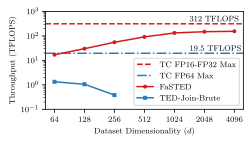
\includegraphics[scale=0.5]{figures/synthetic_flops_comparison.pdf}
    \caption{Tensor Core TFLOPS vs. Dataset Dimensionality}
    \label{fig:tflops_synthetic_comparison}
\end{figure}
\begin{figure}
    \centering
    \includegraphics[scale=0.5]{figures/ExpoDataSpeedVsSize.pdf}
    \caption{\ouralg TFLOPS vs. Dataset Size}
    \label{fig:tflops}
\end{figure}
\begin{figure*}
    \centering
    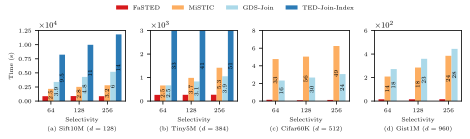
\includegraphics[width=1\textwidth]{figures/RealDataSetSpeedComparison.pdf}
    \caption{Real world dataset comparisons. }
    \label{fig:realworldcomparison}
\end{figure*}
\subsection{Results: Similarity Search Throughput}
In this section, we compare our brute force algorithm, \ouralg, to the index-supported similarity search algorithms on the GPU (\gdsjoin and \tedjoinindex). This is an unfair comparison because \ouralg does not use an index and thus it compares all points to each other, whereas \gdsjoin and \tedjoinindex prune the search to reduce comparing points that are at sufficiently large distances of each other. However, as shown in Section~\ref{sec:eval_throughput}, \ouralg achieves high peak throughput on the tensor cores, and so we evaluate whether it is competitive with the indexed-supported methods.

\begin{table}[!t]
\caption{NVIDIA Nsight Compute profiler results.}
\footnotesize
    \centering
        \begin{tabularx}{\columnwidth}{L|r|r} 
        \hline
             Metric & \ouralg & \tedjoin  \\ \hline
             DRAM Throughput (GB/s) & 152 &  ? \\ \hline
             SMEM Throughput (TB/s) & 2.32  & ?  \\ \hline
             SMEM Bank Conflicts (\%) & 0.0 & ? \\ \hline
             L2 Cache hit rate (\%) &  88 & ? \\ \hline
             Tensor Core Utilization (\%) &  59 & ? \\ \hline
        \end{tabularx}
    \label{tab:profiler_results}
\end{table}

\subsection{Accuracy Comparison}
\begin{table}[!t]
\caption{The accuracy of \ouralg compared to the double precision \gdsjoin algorithm. }
\footnotesize
    \centering
        \begin{tabularx}{\columnwidth}{L|r|r|r|r|r} 
             & \cifar & \gist & \sift & \tinyds \\\hline
             $IoU (\%)$ ($Intersection / Union$)  &  99.96 &  99.99 & 100.0 & 99.98 \\ \hline
        \end{tabularx}
    \label{tab:accuracy}
\end{table}

\section{Discussion \& Conclusions}\label{sec:conclusion}
Discussion points:
-good for smaller $n$ larger $d$?
\brian{Add an discussion about what to consider when running on a different GPU. }
Future work:
-add an index, downside here is that it'll reduce TC utilization. Would need an algorithm design that does not do index searches in the same kernel as TCs.


%Uncomment upon acceptance
% \begin{acks}
% This material is based upon work supported by the National Science Foundation under Grant No. 2042155.
% \end{acks}

%%
%% The next two lines define the bibliography style to be used, and
%% the bibliography file.
\mike{Note: Do a pass over all references including datasets, before submission.}
\bibliographystyle{ACM-Reference-Format}
\bibliography{sample-base}



\end{document}
\endinput
%%
%% End of file `sample-sigconf.tex'.

